\documentclass[
    left=2.5cm,
    right=2.5cm,
    top=2.5cm,
    bottom=3cm,
    bindingoffset=6mm,
    nohyphenation=false
]{szablon/eiti/eiti-thesis}

\usepackage{booktabs}
\usepackage{multirow}
\usepackage{siunitx}
\usepackage{tabularx}   % preambuła
%\usepackage[english]{babel}

\sisetup{detect-all, table-number-alignment=center}
\setlength{\emergencystretch}{3em}

\langpol
\graphicspath{{rysunki/}}
\addbibresource{bibliografia.bib}
\renewcommand{\tablename}{Table}
\renewcommand{\figurename}{Figure}
\renewcommand{\listfigurename}{List of Figures}
\renewcommand{\listtablename}{List of Tables}

% Dodanie usuwa jedno z ostrzeżeń
\usepackage{csquotes}
% Dodanie tego wpływa na wyświetlanie zdjęć w odpowiedni sposób przy adnotacji [H]
\usepackage{float}
\usepackage{subfig}
\usepackage{amsmath}
\usepackage{placeins}
\usepackage{enumitem}
\usepackage{cleveref}
\usepackage{longtable}
\usepackage{makecell}

\begin{document}

\DiplomaThesis
\instytut{Institute of Radioelectronics and Multimedia Technology}
\kierunek{Postgraduate diploma thesis}
\specjalnosc{Deep Learning - Applications in Digital Media}
\title{
    Graph neural networks in medical knowledge graphs
}
\engtitle{
    Graph neural networks in medical knowledge graphs
}
\author{Marta, Monika}
\album{XXXX}
\promotor{YYYYY}
\date{\the\year}
\maketitle

\input{rozdzialy/StreszczeniePL}
\input{rozdzialy/StreszczenieEN}

% Oświadczenie o autorstwie
\cleardoublepage  % Zaczynamy od nieparzystej strony
\pagestyle{plain}
\makeauthorship

% Spis treści
\cleardoublepage % Zaczynamy od nieparzystej strony
\tableofcontents

% Rozdziały
\cleardoublepage % Zaczynamy od nieparzystej strony
\pagestyle{headings}
\newpage % Rozdziały zaczynamy od nowej strony.
\acronymlist

\acronym{GNN}{Graph Neural Network}
\acronym{DAG}{Directed Acyclic Graph}
\acronym{HCR}{Hierarchical Correlation Reconstruction}
\acronym{ADR}{Adverse Drug Reaction}
\acronym{AKI}{Acute Kidney Injury}
\acronym{DILI}{Drug-Induced Liver Injury}
\acronym{GAT}{Graph Attention Network}
\acronym{SAGE}{Graph SAGE}
\acronym{RGCN}{Relational Graph Convolutional Network}
\acronym{AUC}{Area Under the Curve}
\acronym{AUPRC}{Area Under the Precision-Recall Curve}
\acronym{PyG}{PyTorch Geometric}
\input{rozdzialy/1-wstep}
\newpage % Rozdziały zaczynamy od nowej strony.
\section{Main objective}

The main objective of this thesis is to demonstrate how knowledge graphs can be
used in the medical domain in combination with experimental data, i.e.,
real-world patient data. The thesis addresses two tasks:
\begin{itemize}[label=\textendash]
    \item \textbf{Task A: Link prediction}, which reconstructs and updates the
    knowledge graph on the basis of real-world patient data;
    \item \textbf{Task B: Patient risk prediction} (a node-classification task),
    which predicts clinical outcomes using the knowledge graph
    and real-world patient data.
\end{itemize}

The two tasks are complementary and could
form a closed-loop approach to patient-centred care in a real-world medical setting. 
Link prediction focused more on sharing medical knowledge between different stakeholders 
(hospitals, clinicians, patients), while risk prediction focuses on the 
individual patient outcomes.
 As shown in Figure \ref{fig:loop}, these two tasks could operate as 
 an iterative process for improving patient care.

\begin{figure}[h]
    \centering
    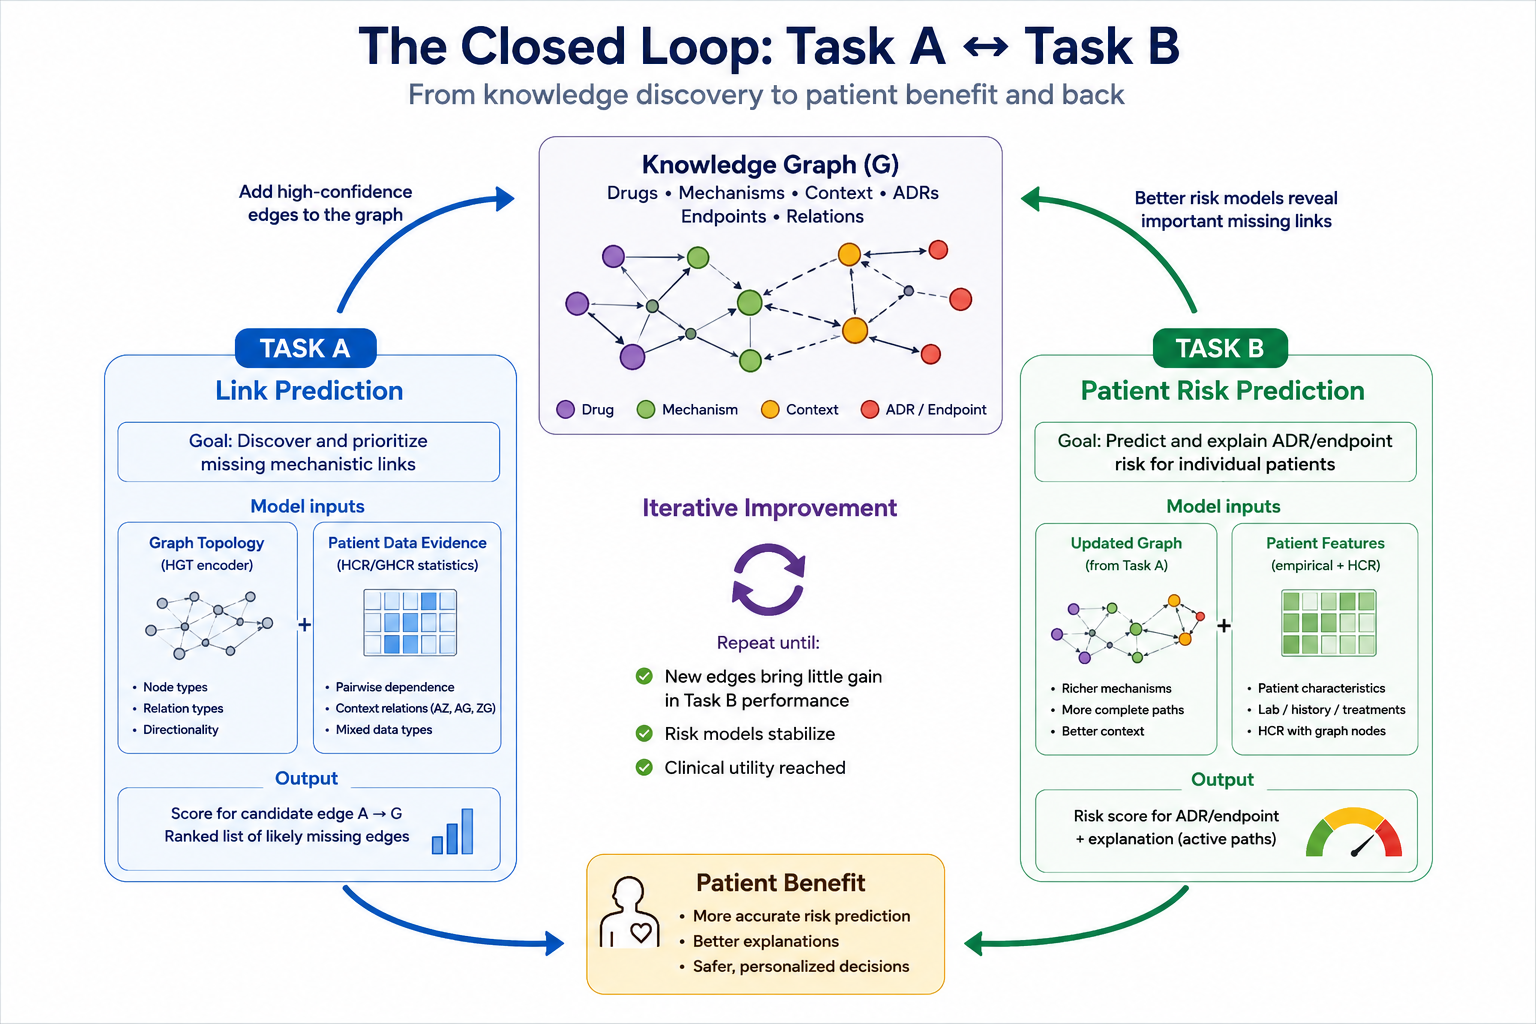
\includegraphics[width=\textwidth, height=0.45\textheight]{rysunki/TASK A i B - loop.png}
    \caption{Overview of the two tasks addressed in this thesis.}
    \label{fig:loop}
\end{figure}
In addition to this domain-oriented objective, the thesis investigates
heterogeneous GNNs enhanced with an additional layer for calculating
dependencies between nodes, namely Hierarchical Correlation Reconstruction
(HCR). This approach examines whether GNNs can be improved by incorporating
statistical dependencies without requiring computationally costly extensions
to the model architecture.
\newpage % Rozdziały zaczynamy od nowej strony.
\section{Related work}

In this section, we review the concepts and methods underlying both tasks
addressed in this thesis: knowledge graphs as structured medical knowledge,
graph neural networks for representation learning on heterogeneous graphs,
and Hierarchical Correlation Reconstruction (HCR) as a statistical complement
to learned graph representations.
We begin with graph-based knowledge representation, then describe deep
learning on graphs, and finally introduce HCR.

\subsection{Knowledge graphs}
\label{subsec:related-kg}

Knowledge graphs represent structured knowledge through entities and the
relations between them.
Formally, a knowledge graph $G$ is a set of triples

\begin{definition}[Knowledge Graph]
\label{def:kg}
$$G \subseteq \mathcal{V} \times \mathcal{R} \times \mathcal{V},$$
where $\mathcal{V}$ denotes the set of entities (nodes) and $\mathcal{R}$
the set of relation types (edge labels). Each triple $(h, r, t) \in G$
corresponds to a directed, labeled edge $h \xrightarrow{r} t$, where $h$
and $t$ are referred to as the head and tail entity, respectively
\textcite{hogan2021knowledge}.
\end{definition}

The key benefit of knowledge graphs is that they provide an interlinked
representation of knowledge in a human- and machine-understandable format
(\textcite{barrasa2023building}).
In biomedical applications, entities may represent drugs, diseases, genes,
proteins, mechanisms, patient characteristics, or clinical outcomes, while
edges describe typed relationships between them.
Such graphs are naturally heterogeneous, because both nodes 
and relations can carry different semantic types.
This motivates the heterogeneous-graph formulation:

\begin{definition}[Heterogeneous Graph]
\label{def:heterokg}
A heterogeneous graph extends Definition~\ref{def:kg} with explicit type
information and is defined as a quadruple
$$G = (V, E, \tau, \phi),$$
where $V$ is the set of nodes, $E \subseteq V \times V$ is the set of
edges, and $\tau: V \rightarrow \mathcal{T}_V$, $\phi: E \rightarrow
\mathcal{T}_E$ are type-mapping functions assigning each node and edge a
type from finite type sets $\mathcal{T}_V$ and $\mathcal{T}_E$
\cite{hu2020heterogeneous}. For an edge $e = (u, v) \in E$, the triple
$\bigl(\tau(u), \phi(e), \tau(v)\bigr)$ defines its schema-level relation,
which corresponds directly to the \texttt{edge\_type} representation used
in the \texttt{HeteroData} object in this thesis.
\end{definition}

Knowledge graphs have been widely applied in biomedical research,
particularly for integrating information from multiple sources and
supporting drug discovery (\textcite{maclean2021knowledge}).
However, many biomedical knowledge graphs primarily encode \emph{associations}
extracted from literature and curated databases, not
patient-specific empirical realizations of the mechanisms they describe.
Popular graph-based methods therefore often ``highlight biological
associations, failing to model causal relationships in complex dynamic
biological systems'' \cite{maclean2021knowledge}.
Recent work has increasingly considered integrating knowledge graphs with
causal or mechanistic representations
\cite{toonsi2025causal,lyu2023causal,mesinovic2026causalgnn}.

Beyond biomedicine, knowledge graphs are also combined with empirical
interaction data in recommendation systems, where models such as KGAT
propagate representations over a collaborative knowledge graph built from
user--item interactions and external knowledge \cite{wang2019kgat}.
The Last-FM benchmark from this line of work is used as a cross-domain
proxy in link prediction task.
The reliability of this benchmark was subsequently questioned by
Shehzad et al.\ \cite{shehzad2025reproducibility} in a reproducibility
study of intent-aware recommendation models; the corrected Last-FM* split
used in this thesis is described in Section~\ref{sec:models-benchmark}.


% Rozdziały zaczynamy od nowej strony.
\subsection{Graphs Neural Networks}

% Graph Neural Networks (GNNs) are types of models that use on how the specific node
% is connected to other nodes in the graph. During training every node is represented 
% by its features and neighbors features that allows not only represent the node based 
% on its own characteristics like it is in traditional neural networks, but also represent
% the node based on its context. This mechanism is called message passing and allows to 
% aggregate information from direct neigbours as well further ones depending on assumed
% number of layers in network. There are multiple types of GNNs that differ from Each
% other based on how the message from neighbors is aggregated. In this Section we 
% review couple of them that were applied in this work.

Graph neural networks (GNNs) are a class of models that leverage how a given node is connected 
to other nodes in the graph. During training, every node is represented not only by its own 
features, as in traditional neural networks, but also by the features of its neighbours.
What it is new in GNNs comparing to previous graph embedding methods is that the representation
is not fixed and it is built based on aggregation, so it is not necessary to have all nodes in the graph 
during training. 
%fixed representation for every node observed during training, making it impossible to 
%generate embeddings for nodes that did not appear in the training graph. 
%This allows the node's representation to capture its surrounding context in addition to its own 
%characteristics. 
This mechanism, known as message passing, aggregates information from direct 
neighbours as well as from more distant ones, depending on the number of layers assumed in the 
network. GNN  builds a node's representation at each layer by combining its own representation from
the previous layer with the aggregated representations of its neighbors, also from the 
previous laye
Formally, the representation $h_v^{(K)}$ of node $v$ depends on
the features of all nodes within its $K$-hop neighborhood.
Since each layer $k$ updates
\begin{equation}
h_v^{(k)} = \text{UPDATE}\Bigl(h_v^{(k-1)},\ \text{AGGREGATE}\bigl(\{h_u^{(k-1)} : u \in \mathcal{N}(v)\}\bigr)\Bigr),
\end{equation}
so that information from a node $u$ at graph distance $d$ from $v$ only reaches $v$ once $K \geq d$.
Different types of GNNs differ primarily in how they aggregate messages from their 
neighbors. In this section, we review several such architectures that were applied in this work.

--dodanie informacji o wagach modelu i jak tworzona reprezentacja / embedding 

\subsubsection{GraphSAGE}

  GraphSAGE \cite{hamilton2017inductive} was introduced in response to the need for inductive 
  and scalable representation learning on graphs. As introduced in this section introduction, 
  GraphSAGE instantiates the general message-passing scheme using one of three 
  aggregation functions — mean, LSTM, or pooling — so that the same learned functions can later 
  be applied to any node.
  What is specific to GraphSAGE is that the node's own representation and the aggregated 
  neighbor representation are concatenated into single and longer vector, 
  and the resulting vector is L2-normalized after each layer.
  Additionally, GraphSAGE addresses the scalability of training by sampling a fixed number of 
  neighbors for each node, not full neighbourhood,
  and updating the node's representation based on this sampled subset.

\subsubsection{Relational Graph Convolutional Network}

Relational Graph Convolutional Networks (R-GCNs) \cite{schlichtkrull2018modeling}
extend Graph Convolutional Networks (GCNs) to multi-relational graphs, in
which edges represent different types of relationships. Unlike a
standard GCN, which applies the same transformation to messages from all
neighbours, R-GCN applies a relation-specific transformation. 

For a node $v$, the representation at layer $l+1$ is computed as

\begin{equation}
\label{eq:rgcn}
h_v^{(l+1)} =
\sigma \left(
\sum_{r \in \mathcal{R}}
\sum_{u \in \mathcal{N}_r(v)}
\frac{1}{c_{v,r}}
W_r^{(l)} h_u^{(l)}
+
W_0^{(l)} h_v^{(l)}
\right),
\end{equation}

where $\mathcal{R}$ is the set of relation types,
$\mathcal{N}_r(v)$ denotes the set of neighbours connected to node $v$
through relation $r$, $W_r^{(l)}$ is a trainable weight matrix specific to
relation $r$, and $c_{v,r}$ is a normalisation constant. The term
$W_0^{(l)} h_v^{(l)}$ represents a self-loop transformation, which preserves
the node's own representation in addition to messages received from its
neighbours. Finally, $\sigma$ denotes a non-linear activation function.

When the number of relation types is large, assigning a separate full
weight matrix to each relation can lead to a large number of parameters and overfitting.
To address this issue, R-GCN introduces basis decomposition, in which each
relation-specific matrix is expressed as a linear combination of $B$ shared
basis matrices:

\begin{equation}
\label{eq:rgcn-basis}
W_r^{(l)} =
\sum_{b=1}^{B} a_{rb}^{(l)} V_b^{(l)},
\end{equation}

where $V_b^{(l)} \in
\mathbb{R}^{d_{\mathrm{out}} \times d_{\mathrm{in}}}$ is the $b$-th shared
basis matrix and $a_{rb}^{(l)}$ is a trainable coefficient specifying the
contribution of this basis to relation $r$. 

\subsubsection{Transformed-based GNN}

Transformer-based graph neural networks adapt the self-attention mechanism
introduced in the Transformer architecture (\textcite{vaswani2017attention}) to
graph-structured data.
Instead of using a fixed type of aggregation of neighbours information,
the architecture uses an attention-based message passing mechanism that allows 
to recognize the importantance of neighbouring nodes.
For each node $i$, its input representation $\mathbf{h}_i$ is designed by a projections:
query, key and value:
\begin{equation}
\mathbf{q}_i = \mathbf{W}_{Q}\mathbf{h}_i, \qquad
\mathbf{k}_i = \mathbf{W}_{K}\mathbf{h}_i, \qquad
\mathbf{v}_i = \mathbf{W}_{V}\mathbf{h}_i,
\end{equation}
where $\mathbf{W}_{Q}$, $\mathbf{W}_{K}$, and $\mathbf{W}_{V}$ are learnable
weight matrices.
Then for an edge from a source node $j$ to a target node $i$, the weight of attention 
(attention coefficient) is calculated based on equation:
\begin{equation}
    e_{ij} =
    \frac{\mathbf{q}_{i}^{\top}\mathbf{k}_{j}}{\sqrt{d_k}},
    \end{equation}
    where $d_k$ denotes the dimensionality of the key vectors.

The attention coefficients are normalised across all neighbours $\mathcal{N}(i)$ of the target
    node using the softmax function:
    \begin{equation}
    \alpha_{ij} =
    \frac{\exp(e_{ij})}
    {\sum_{r \in \mathcal{N}(i)} \exp(e_{ir})}.
    \end{equation}
The node's representation is updated by aggregating value projections of
its neighbours, weighted by the learned attention coefficients:
\begin{equation}
\mathbf{h}'_i =
\sum_{j \in \mathcal{N}(i)}
\alpha_{ij}\mathbf{v}_{j}.
\end{equation}

To capture multiple complementary patterns of neighbourhood interactions, Graph
Transformers commonly use multi-head attention. For each attention head
$m \in \{1, \ldots, H\}$, independent projection matrices
$\mathbf{W}_{Q}^{(m)}$, $\mathbf{W}_{K}^{(m)}$, and
$\mathbf{W}_{V}^{(m)}$ are learned. The output of head $m$ for node $i$ is:
\begin{equation}
\mathbf{h}_i^{\prime(m)} =
\sum_{j \in \mathcal{N}(i)}
\alpha_{ij}^{(m)}\mathbf{v}_{j}^{(m)}.
\end{equation}
The outputs of all $H$ heads are combined by concatenating or averaging them.
This mechanism provides a trainable aggregation methods, not defined by default like in previously mentioned
architectures.

All architectures mentioned in this section can be applied to heterogeneous
graphs through an appropriate configuration of the \texttt{HeteroConv} layer in
PyTorch Geometric (PyG). \texttt{HeteroConv} is a generic wrapper that applies
a separately specified message-passing operator to each edge type, i.e., each
meta-relation between a source node type and a target node type
\textcite{wojcik2026grafowe}.

For attention-based message passing in heterogeneous graphs, a dedicated
architecture called the Heterogeneous Graph Transformer (HGT) was proposed 
 in \textcite{hu2020heterogeneous}.
HGT makes attention scores and message transformations dependent on the
types of source and target nodes and on the edge relation type.

For an edge from a source node $s$ to a target node $t$, HGT represents its
semantics as a meta-relation
$(\tau_s, \phi(e), \tau_t)$, where $\tau_s$ and $\tau_t$ denote the source
and target node types, respectively, and $\phi(e)$ denotes the edge type.
The target node produces a query, whereas the source node produces a key and
a value. Relation-specific transformations affect both the attention score and
the message transferred from $s$ to $t$.

Consequently, HGT can assign different importance to neighbours depending not
only on their features, but also on the semantic type of their connection to
the target node. The weighted incoming messages are then aggregated and
transformed using parameters specific to the target node type. 

%\subsubsection{Depth of GNNs}
% Residual connections switch the effective per-layer propagation operator from the
% (nilpotent, on a DAG without self-loops) 
% adjacency operator , which is the standard formalization of the over-smoothing regime and is the mechanism 
% through which multi-layer signal survives on a directed acyclic structure.

% PairNorm (Zhao et Akoglu, 2020) re-centers and re-scales node representations after each layer to keep the pairwise distance between representations from collapsing, without preventing the underlying mixing.

% DropEdge (Rong et al., 2020) randomly removes a fraction of edges independently in every layer during training, slowing the rate of information mixing and acting as a structural regularizer.

% Jumping Knowledge (Xu et al., 2018) aggregates the outputs of all layers (via concatenation, cat, or elementwise max) rather than only the last one, letting a node fall back on a shallower, less-smoothed representation when the deepest layer has become uninformative.

% Weisfeiler-Lehman --- two nodes with identical initial features and structurally equivalent neighborhoods 
% cannot be assigned distinct representations by any number of convolutional layers.

% leave-one-out
\newpage % Rozdziały zaczynamy od nowej strony.
\subsection{HCR}
\label{subsec:hcr_def}

\subsubsection{Hidden link reconstuction}

\subsubsection{Endpoint prediction}

Endpoint prediction is a node classification tasks in data. 


% % Rozdziały zaczynamy od nowej strony.
\subsection{Evaluation Metrics}
\label{subsubsec:metrics}

The proposed models were evaluated using the area under the receiver operating
characteristic curve (AUC), the area under the precision--recall curve (AUPRC),
and the Lift measure. As the synthetic dataset generated for this project contains
rare events and class imbalance, AUPRC was included as an additional performance
metric because it focuses on the positive class and reflects the trade-off
between precision and recall. Below there included the equations for calculating metrics.

\emph{AUC} is the area under the receiver operating characteristic curve (ROC-AUC) 
and is defined as:
\begin{equation}
  \mathrm{ROC\mbox{-}AUC}
  =
  \int_0^1 \mathrm{TPR}(\mathrm{FPR})\,d\mathrm{FPR}.
  \end{equation}
  where $\mathrm{TPR}$ is the true positive rate and $\mathrm{FPR}$ is the false positive rate.

\emph{AUPRC} is the area under the precision--recall curve and is defined as:
\begin{equation}
  \mathrm{AP} =
  \sum_{n}
  \left(R_n - R_{n-1}\right) P_n,
  \end{equation}
  where $P_n$ and $R_n$ denote precision and recall at the $n$-th threshold,
  respectively.

\emph{Lift} is the AUPRC divided by the prevalence baseline, that is, the
factor by which the model improves over a random ranking, e.g. at a mean
prevalence of $5.5\%$ a lift of $2.3$ corresponds to an AUPRC of $0.125$.

In addition to the traditional metrics described above, a
\emph{generator-based oracle AUC} was computed for the node-classification
task. Because the dataset is synthetic, the logistic generative model for
each endpoint is known: each patient is scored with the true parent effects
from the audited DAG and ROC-AUC is evaluated on the resulting
probabilities. Model performance is reported relative to this reference via
\emph{\% of oracle AUC}:

\begin{equation}
  \frac{\mathrm{AUC} - 0.5}{\mathrm{AUC}_{\mathrm{Oracle}} - 0.5} \cdot 100\%,
  \label{eq:pct-ceiling}
\end{equation}
%
where $\mathrm{AUC}_{\mathrm{Oracle}} = 0.651$ is the macro-averaged oracle
AUC over the same eight endpoints used in aggregate reporting. This metric
expresses the share of ranking signal recoverable under the known generator,
relative to random performance at $0.5$.



\newpage % Rozdziały zaczynamy od nowej strony.
\section{Dataset}

Deep learning research on medical knowledge graphs currently leaves two related
 gaps unaddressed. First, causal modeling is rarely applied at the level of 
 the full patient trajectory.
 Second, most knowledge graphs encode relationships extracted from literature, 
 without integrating patient-level empirical data on how outcomes are actually 
 observed (as well noted by \textcite{toonsi2025causal}). 
 To address both gaps, we generated a synthetic dataset that jointly 
 encodes a known causal structure and its patient-level empirical realizations, 
 providing ground truth for both link prediction and node classification. 
 This gave a full control over how knowledge is encoded in the graph, 
 avoiding reconstruction from a partially observed real-world dataset.
 The generation process, the resulting graph, and the derived patient data are 
 described in detail in this chapter. 
 
 Additionally, there is included 
 a description of benchmark datasets used for testing the prototyped models.

\subsection{Synthethic dataset}

The dataset includes two structures:

\begin{enumerate}
    \item a causal knowledge graph (DAG) that encodes causal patient pathways
    from patient characteristics and drug exposures to clinical events
    (endpoints);
    \item an empirical dataset --- a patient-level table with each patient's
    characteristics and observations, generated from the knowledge graph
    (Section~\ref{subsec:generation}).
\end{enumerate}

\subsubsection{Knowledge graph}

The construction of the knowledge graph started from defining the clinical
endpoints to model and predict, and identifying which patient
characteristics and drug exposures are known to influence them. This
approach -- starting from the target and working backwards to its
determinants -- was chosen so that every path in the graph corresponds to a
patient clinical pathway.

As our team includes a team member with a pharmacology background, her
domain knowledge was used for constructing and verifying the initial version
of the knowledge graph -- the first set of endpoints, risk factors, and
drug classes. Candidate mechanistic pathways connecting a drug exposure to a
given endpoint, including specific drug-drug and drug-disease interaction
gates, were proposed with the support of
Fable\footnote{Fable refers to Claude Fable 5, a large language model
developed by Anthropic, which was used as an AI-assisted modelling aid to
draft candidate mechanistic pathways for review.}. All proposals generated
with its support were accepted, rejected, or modified by the team member
with a pharmacology background before being incorporated into the graph
specification.

The graph was built iteratively. An initial, smaller version of the DAG
covered a limited set of drug classes, 
mechanisms, and endpoints. Once this core structure was
validated, it was progressively extended with
additional nodes and edges. The final version includes 155 nodes organised
into six layers specified in Tables ~\ref{tab:node_types} and 405 directed edges grouped into categories in 
~\ref{tab:edge_type_categories}.

\begin{table}[htbp]
    \centering
    \caption{Node types in the patient causal DAG.}
    \label{tab:node_types}
    \begin{tabularx}{\textwidth}{@{}l X@{}}
        \toprule
        \textbf{Node type} & \textbf{Description} \\
        \midrule
        \texttt{patient\_context} & Patient-level covariates (e.g. demographics, comorbidities). \\
        \addlinespace
        \texttt{drug\_exposure} & Drugs the patient is exposed to. \\
        \addlinespace
        \texttt{mechanism} & Intermediate physiological mechanisms mediating the effect of a drug or context on further stages. \\
        \addlinespace
        \texttt{adr\_or\_intermediate\_state} & Intermediate adverse or physiological states positioned between mechanisms and clinical endpoints. \\
        \addlinespace
        \texttt{observation\_or\_selection} & Nodes representing observation, documentation, or selection processes rather. \\
        \addlinespace
        \texttt{clinical\_endpoint} & Target adverse clinical outcomes (e.g. AKI, DILI, Hospitalization). \\
        \bottomrule
    \end{tabularx}
\end{table}


\begin{figure}[h]
    \centering
    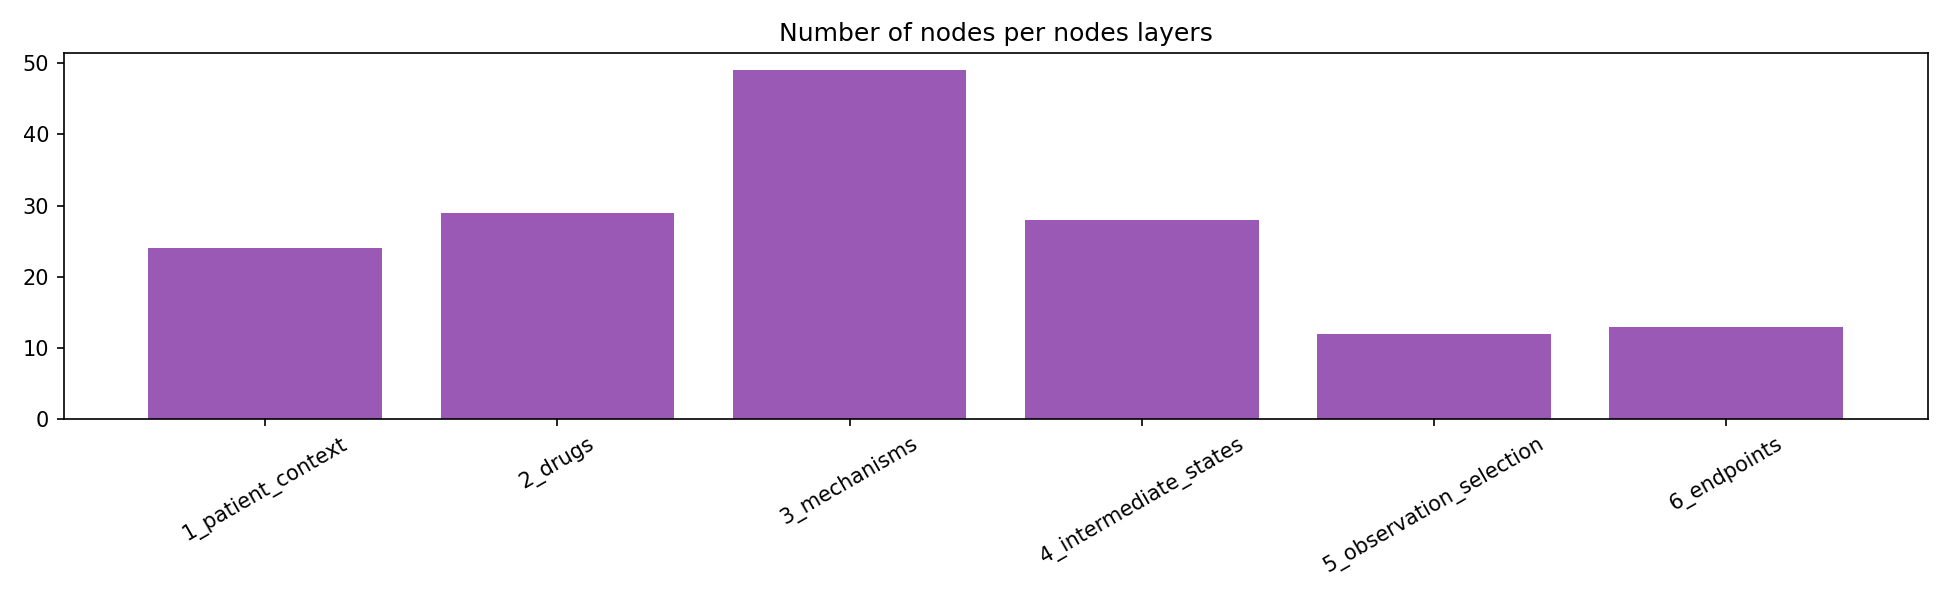
\includegraphics[width=\textwidth, height=0.45\textheight, keepaspectratio]{rysunki/01_node_counts_by_type_and_layer.png}
    \caption{Frequency of nodes types.}
    \label{fig:architecture}
\end{figure}

Beyond its topology, every node in the graph carries a set of attributes
which are used directly in the
data-generating process described in Section~\ref{subsec:generation}:

\begin{itemize}
    \item \texttt{base\_prevalence} encodes a population-level
    probability of a node being present in a patient who has none of the
    node's risk factors active.
    \item \texttt{severity\_weight} encodes the clinical severity assigned to
    a node, independent of how frequently it occurs.
    \item \texttt{observability} encodes how reliably a true clinical state is
    expected to be recorded in practice.
\end{itemize}

\begin{table}[htbp]
    \centering
    \small
    \setlength{\tabcolsep}{5pt}
    \renewcommand{\arraystretch}{1.2}
    \caption{Semantic categories of directed edges in the patient causal DAG.}
    \label{tab:edge_type_categories}

    \begin{tabular}{@{}p{0.30\textwidth} p{0.64\textwidth}@{}}
        \toprule
        \textbf{Category} & \textbf{Included edge types} \\
        \midrule

        Background risk and treatment assignment &
        \makecell[l]{
            \texttt{risk\_modifier}, \texttt{confounding},\\
            \texttt{latent\_confounding}, \texttt{treatment\_indication},\\
            \texttt{treatment\_burden}
        } \\
        \addlinespace[3pt]

        Drug effects and mechanistic pathways &
        \makecell[l]{
            \texttt{drug\_to\_mechanism}, \texttt{causal\_mechanistic},\\
            \texttt{mechanism\_to\_adr}, \texttt{adr\_to\_intermediate}
        } \\
        \addlinespace[3pt]

        Clinical outcome progression &
        \makecell[l]{
            \texttt{adr\_to\_endpoint},\\
            \texttt{endpoint\_to\_hospitalization}
        } \\
        \addlinespace[3pt]

        Observation and selection processes &
        \makecell[l]{
            \texttt{observation}, \texttt{selection},\\
            \texttt{observation\_process}
        } \\
        \addlinespace[3pt]

        Polypharmacy, aggregate burden, and interactions &
        \makecell[l]{
            \texttt{drug\_to\_burden}, \texttt{drug\_to\_load},\\
            \texttt{interaction\_gate\_component},\\
            \texttt{drug\_pairwise\_gate}, \texttt{drug\_triple\_gate},\\
            \texttt{interaction\_amplify},\\
            \texttt{adr\_burden\_component}, \texttt{burden\_threshold}
        } \\
        \bottomrule
    \end{tabular}
\end{table}

As edges bring different information based on edge type, they were assigned declared attributes, such as:

\begin{itemize}
    \item \texttt{effect\_size} encodes the strength of the causal effect of
    the source node on the target node.
    \item \texttt{effect\_sign} encodes the direction of that effect
    (risk-increasing or risk-decreasing).
\end{itemize}

In \cref{fig:dag_overview} it is visualized an overview of DAG graph. 

\begin{figure}[h]
    \centering
    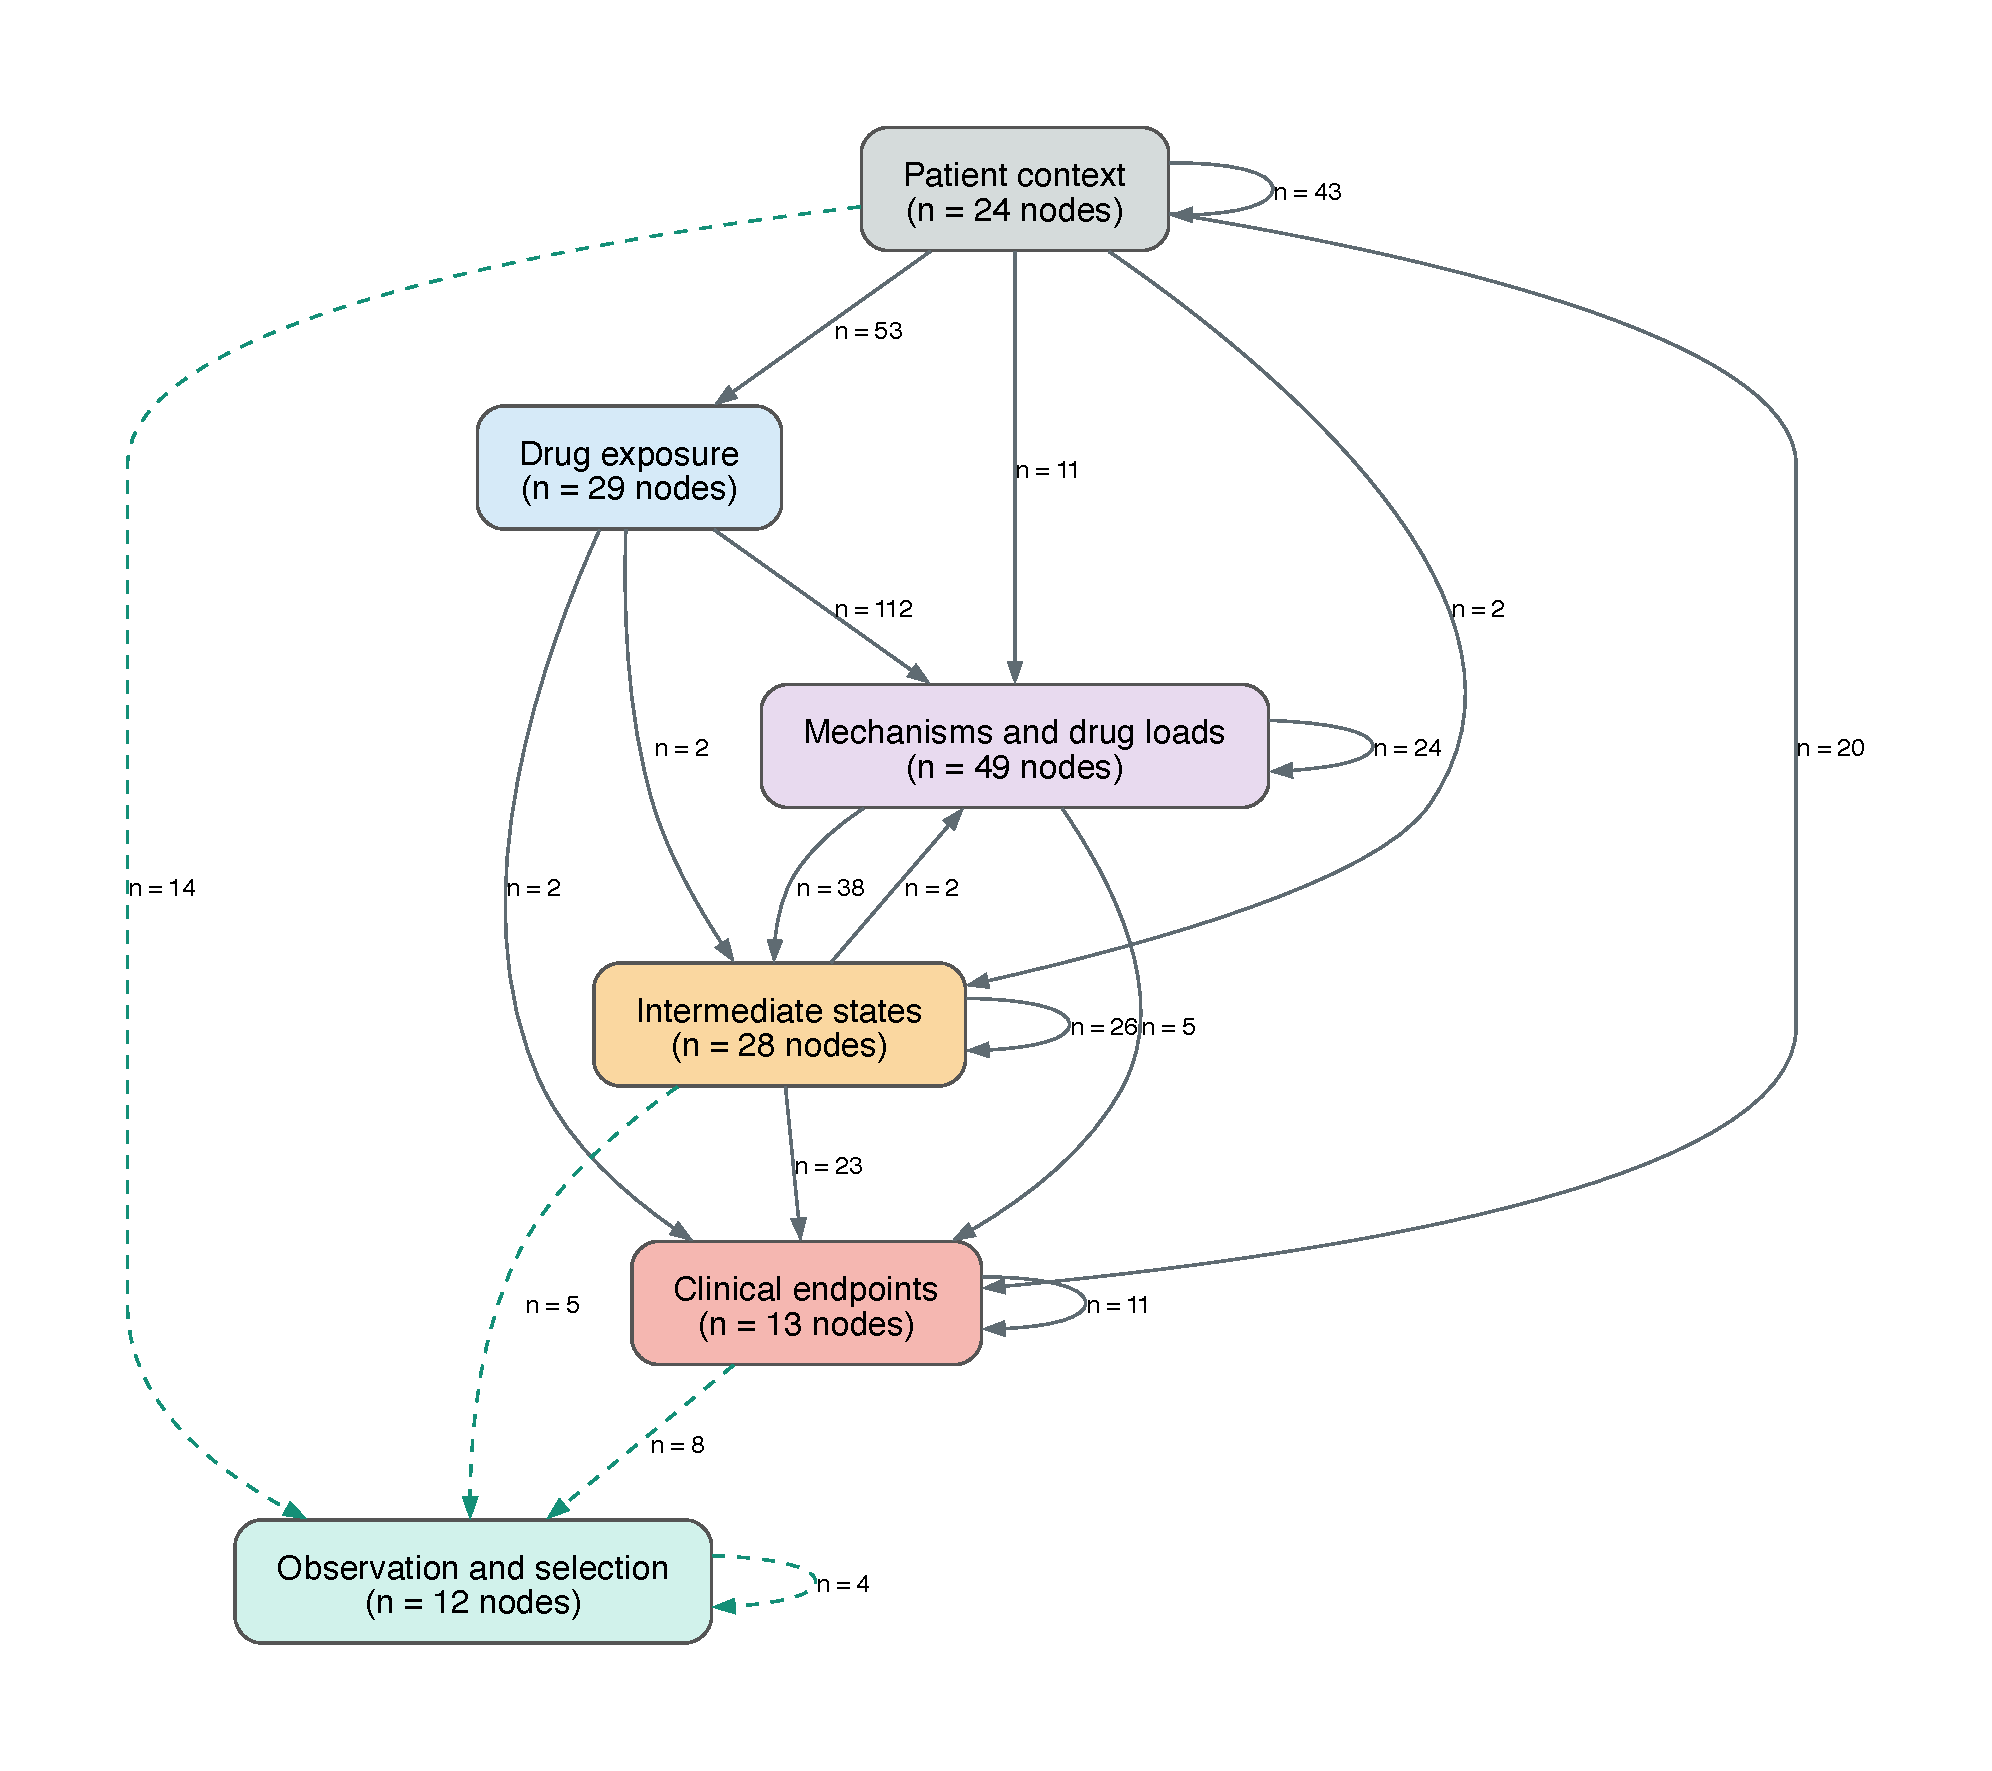
\includegraphics[width=\textwidth, height=0.45\textheight, keepaspectratio]{rysunki/causal_dag_type_overview.pdf}
    \caption{DAG visualization}
    \label{fig:dag_overview}
\end{figure}

The final version of the DAG was verified statistically with the metrics
reported in \cref{tab:dag_structural_stats}. They confirm the graph's
acyclicity and characterize its structural complexity for modelling
purposes.

\begin{table}[htbp]
    \centering
    \caption{Structural statistics of the causal knowledge graph.}
    \label{tab:dag_structural_stats}
    \begin{tabularx}{\textwidth}{@{}l X@{}}
        \toprule
        \textbf{Metric} & \textbf{Value} \\
        \midrule
        Nodes / edges & 155 / 405 \\
        Graph density & 0.017 \\
        Acyclicity  & True \\
        Self-loops / duplicate edges & 0 / 0 \\
        Source nodes / sink nodes & 9 / 12 \\
        Direct parents per clinical endpoint & mean 4.7 (range 1--14) \\
        Ancestors per clinical endpoint & median 31 (range 9--126) \\
        Longest root-to-endpoint path & median 12 edges (range 5--16) \\
        Shortest root-to-endpoint path & 1 edge for 10 of 13 endpoints; 3--4 edges for the three rarest endpoints \\
        %Causal motifs (mediation / fork / collider) & 922 / 1{,}545 / 1{,}022 triplets \\
        Drug--endpoint pairs sharing a common ancestor & 85 \\
        \bottomrule
    \end{tabularx}
\end{table}

% It is worth to mention that DAG includes 
% an unobserved confounder \texttt{unobserved\_severity} that accounts for 741 of the
% 1{,}545 fork triplets in the graph (48\%) -- that's why it is recommended for exclusion
% on the 
%  Second, the three
% endpoints with the lowest Bayes ceiling (Section~\ref{sec:generation}) --
% serotonin syndrome, rhabdomyolysis, and lactic acidosis -- are exactly the
% three endpoints with a single direct parent and the longest minimum
% root-to-endpoint distance (3--4 edges, versus 1 edge for all other
% endpoints). This is a purely structural property, observable without
% generating a single patient, and it independently corroborates the
% distributional finding reported later in this chapter.


\subsubsection{Patient data}
\label{subsec:generation}

The patient-level data generation procedure was designed to produce
tabular records that provide empirical evidence for knowledge-graph
reconstruction and downstream prediction of clinical outcomes. Its purpose
was to transform the static causal DAG specification into a patient-level
dataset in which each individual is represented by a realised configuration
of exposures, clinical states, and outcomes. This enables the graph
representation to be used as a dynamic, data-supported structure for
multiple downstream tasks.
For each of 20{,}000 simulated patients, the generator assigns a realised
value to each of the 155 nodes in the causal DAG. Values are generated in
topological order, following the causal direction of the graph. For every
patient, upstream context variables are generated first, followed by drug
exposures, physiological mechanisms, and intermediate adverse states.
Clinical endpoints are generated only after all their parent variables have
been realised.
Each node value is generated by one of three mechanisms:
a stochastic process, a deterministic computation of other nodes, or a
deterministic observation rules. The following paragraphs
describe each mechanism.

\paragraph{Stochastic nodes}
Most nodes -- patient covariates, drug exposures, intermediate mechanisms,
and clinical endpoints -- are generated as Bernoulli draws whose probability
is a logistic function of their parents:

\begin{equation}
\eta_i = \operatorname{logit}(p_i^{0}) + \sum_{j \in \mathrm{parents}(i)} s_{ij} \cdot w_{ij} \cdot x_j,
\qquad
x_i \sim \mathrm{Bernoulli}\big(\sigma(\eta_i)\big),
\end{equation}

where $p_i^{0}$ is the node's baseline prevalence, $x_j$ is the realised
value of parent $j$, and $w_{ij}$, $s_{ij}$ are the effect size and effect
sign declared on the edge $j \to i$. Nodes are generated in topological
order, so that every parent has already been assigned a value before its
children are processed.

Three conditions affect the implementation:

\begin{itemize}
    \item A parent with more than two distinct realised values (i.e.\ a
    \texttt{count} or \texttt{continuous} node, such as
    \texttt{polypharmacy\_burden}) is standardised before entering
    the sum, $(x_j - \bar{x}_j) / \mathrm{sd}(x_j)$, so that its
    contribution to $\eta_i$ is on a comparable scale to binary parents.
    \item $p_i^{0}$ is taken from the \texttt{base\_prevalence} column of
    the node specification \footnote{If base prevalence value is missing, a type-dependent
    default is used instead (0.16 for drug exposures, 0.02 for clinical
    endpoints, 0.35 for observation/selection nodes, 0.10 otherwise)}.
    \item  If missing, \texttt{effect\_size}, and
    \texttt{effect\_sign} defaults to 0.5 and $+1$ accordingly.
\end{itemize}

\paragraph{Deterministic derived variables.}

Some variables are derived deterministically from values that have already been
generated based on  patterns of polypharmacy, drug interactions, and
adverse-event burden explicit in the graph.

Table~\ref{tab:deterministic_variables} summarises the deterministic
variables and their generating rules. 
%The complete variable-level
%data-generating specification is provided in
%Appendix~\ref{app:data_generating_spec}.

\begin{table}[htbp]
    \centering
    \small
    \caption{Deterministic variables in the synthetic patient generator.}
    \label{tab:deterministic_variables}
    \begin{tabularx}{\textwidth}{@{}
        p{0.33\textwidth}
        p{0.18\textwidth}
        X@{}}
        \toprule
        \textbf{Variable group} &
        \textbf{Rule type} &
        \textbf{Generating rule} \\
        \midrule

        Renal, CNS, bleeding, serotonergic, and hepatic
        \texttt{ddi\_*} gates &
        Conjunctive gate &
        A binary variable equal to 1 only when all listed drug-exposure
        components are active. For example,
        \texttt{ddi\_renal\_triple\_whammy}
        $= \texttt{nsaid} \land \texttt{acei\_arb} \land
        \texttt{diuretic}$. \\

        \addlinespace
        Drug--disease interaction gates
        (\texttt{drug\_disease\_*}) &
        Conjunctive gate &
        A binary variable equal to 1 when the relevant drug exposure or drug
        load and the associated patient risk factor are both active. \\

        \addlinespace
        \texttt{active\_drug\_count} &
        Drug count &
        Sum of all 29 binary \texttt{drug\_exposure} variables. \\

        \addlinespace
        Drug-load variables
        (\texttt{nephrotoxin\_load}, \texttt{hepatic\_drug\_load},
        \texttt{qt\_drug\_load\_v3}, \texttt{cns\_depressant\_load},
        \texttt{bleeding\_risk\_load}, \texttt{serotonergic\_load},
        \texttt{cyp\_inhibitor\_load}) &
        Drug count &
        Sum of active drug exposures belonging to a predefined clinical risk
        group. \\

        \addlinespace
        \texttt{ddi\_qt\_multidrug\_load} &
        Drug count &
        Sum of active QT-prolonging drug exposures specified in the
        generator. \\

        \addlinespace
        \texttt{ddi\_serotonergic\_high\_load} &
        Threshold &
        Equal to 1 when \texttt{serotonergic\_load} is at least 2. \\

        \addlinespace
        \texttt{cumulative\_adr\_burden} &
        Weighted sum &
        Severity-weighted sum of intermediate adverse states plus
        $0.08 \times \texttt{active\_drug\_count}$. \\

        \addlinespace
        \texttt{severe\_adr\_burden} &
        Threshold &
        Equal to 1 when \texttt{cumulative\_adr\_burden} is at least 4.0. \\

        \bottomrule
    \end{tabularx}
\end{table}

\paragraph{Deterministic observation rules}

A small set of variables is generated deterministically as the product of an
underlying clinical state and its associated observation process. For
example,

\[
\texttt{elevated\_creatinine\_recorded}
=
\texttt{creatinine\_rise}
\times
\texttt{creatinine\_tested}.
\]

These variables represent recorded clinical evidence rather than the
underlying patient state alone. Thus, a creatinine rise may be present but
remain absent from the recorded data if no creatinine test is performed.
Analogous deterministic rules are applied to recorded ALT/AST elevation and
recorded QT prolongation.

The observation variables distinguish clinical truth from documentation and
are retained as part of the complete data-generating process. They also
provide a structured representation of testing and recording mechanisms that
is relevant to the construction and interpretation of alternative
observational scenarios.


\subsubsection{Evaluation scenarios}



Data was generated in five controlled
scenarios constructed to evaluate model robustness under common
challenges of observational clinical data. All scenarios use the same
underlying synthetic pharmacotherapy DAG and preserve the semantic meaning of
node and edge types. Each scenario modifies either the available information,
the sampling mechanism, the treatment-assignment process, the observation
process, or the institutional context. 

For example, the \texttt{selectionbias} scenario restricts the cohort to
patients with hospital contact, creatinine testing, and liver-function
testing. Consequently, inclusion depends on downstream healthcare-contact
and diagnostic processes. The observation and documentation variables therefore support
interpretation of this scenario.

All of scenarios are presented in Table ~\ref{tab:synthethic_scenarios}.

\begin{table}[htbp]
    \centering
    \small
    \caption{Synthetic evaluation scenarios and their intended data challenge.}
    \label{tab:synthetic_scenarios}
    \begin{tabularx}{\textwidth}{@{}l X@{}}
        \toprule
        \textbf{Scenario} & \textbf{Primary purpose} \\
        \midrule
        \texttt{clean} &
        Reference setting with complete generated information. \\
        \addlinespace

        \texttt{hidden\_confounder} &
        Unmeasured confounding: \texttt{unobserved\_severity} remains active
        in the generator but is withheld from the observed data. \\
        \addlinespace

        \texttt{selection\_bias} &
        Selection bias induced by restricting the cohort to patients with
        hospital contact, creatinine testing, and liver-function testing. \\
        \addlinespace

        \texttt{no\_overlap} &
        Positivity violation caused by subgroup-specific treatment
        probabilities. \\
        \addlinespace

        \texttt{noisy\_documentation} &
        Imperfect clinical recording, including false negatives and a 1\%
        false-positive recording probability. \\
        \addlinespace

        \texttt{multihospital} &
        Institutional heterogeneity in treatment assignment and documentation
        processes across four synthetic hospitals. \\
        \bottomrule
    \end{tabularx}
\end{table}

\subsubsection{Resulting patient-level dataset}

Th final dataset generated
contains 20{,}000 simulated patients for every scenario described. Each row represents one patient and
each graph node is represented by a corresponding patient-level variable.
Table~\ref{tab:patient_dataset_schema} summarises the structure and value
types of the resulting dataset. A complete variable-level data dictionary is
provided in Appendix~\ref{appendix-list}.

\begin{table}[htbp]
    \centering
    \caption{Schema of the generated patient-level dataset.}
    \label{tab:patient_dataset_schema}
    \begin{tabularx}{\textwidth}{@{}X c X@{}}
        \toprule
        \textbf{Variable group} &
        \textbf{Number} &
        \textbf{Value type} \\
        \midrule

        \texttt{patient\_id} &
        1 &
        Integer identifier. \\

        \addlinespace
        \texttt{hospital\_id} &
        1 &
        Categorical integer identifier. \\

        \addlinespace
        \texttt{patient\_context} &
        24 &
        Mostly binary; selected count and baseline-measurement variables. \\

        \addlinespace
        \texttt{drug\_exposure} &
        29 &
        Binary. \\

        \addlinespace
        \texttt{mechanism} &
        49 &
        Binary, count, and deterministic gate variables. \\

        \addlinespace
        \texttt{adr\_or\_intermediate\_state} &
        28 &
        Mostly binary; derived score and threshold variables. \\

        \addlinespace
        \texttt{observation\_or\_selection} &
        12 &
        Binary. \\

        \addlinespace
        \texttt{clinical\_endpoint} &
        13 &
        Binary. \\

        \bottomrule
    \end{tabularx}
\end{table}

\texttt{Clinical endpoints}

The 13 clinical endpoints are binary stochastic variables generated after
their direct parents have been realised. Their values are the ground-truth
labels used for endpoint prediction. Table~\ref{tab:app_endpoints} lists the
endpoint names and their direct parents in the final DAG.

\begin{table}[htbp]
    \centering
    \small
    \caption{Endpoint prevalence and AUROC ceiling in the evaluation subset.}
    \label{tab:app_endpoints}
    \begin{tabular}{lrrrr}
        \toprule
        \textbf{Endpoint} &
        \textbf{Positive cases} &
        \textbf{Prevalence (\%)} &
        \textbf{AUROC ceiling (\%)} &
        \textbf{Parents} \\
        \midrule
        AKI                 & 393 & 13.10 & 81.13 & 6 \\
        DILI                & 55  & 1.83  & 65.29 & 7 \\
        Delirium            & 111 & 3.70  & 66.80 & 4 \\
        Depression          & 254 & 8.47  & 65.25 & 6 \\
        Falls               & 234 & 7.80  & 69.67 & 7 \\
        GI bleeding         & 64  & 2.13  & 57.04 & 5 \\
        Hospitalization     & 676 & 22.53 & 75.07 & 14 \\
        Hyperkalemia        & 146 & 4.87  & 58.98 & 2 \\
        Hyponatremia        & 236 & 7.87  & 63.83 & 3 \\
        QT arrhythmia       & 48  & 1.60  & 62.24 & 4 \\
        Serotonin syndrome  & 8   & 0.27  & 55.45 & 1 \\
        Rhabdomyolysis      & 11  & 0.37  & 53.02 & 1 \\
        Lactic acidosis     & 17  & 0.57  & 52.32 & 1 \\
        \bottomrule
    \end{tabular}
\end{table}

\paragraph{Patient-level data splits}

Patients were partitioned into mutually exclusive training, validation, and
test sets in proportions of 70\%, 15\%, and 15\%, respectively. For the
\texttt{clean} scenario containing 20{,}000 patients, this corresponds to
14{,}000 training patients, 3{,}000 validation patients, and 3{,}000 test
patients.

Splits were created at the \texttt{patient\_id} level using a deterministic
greedy multi-label balancing procedure with seed \texttt{20260722}. Patients
with rare endpoint combinations were assigned first, and assignments were
chosen to preserve the prevalence of each clinical endpoint across the three
splits. Consequently, every patient appears in exactly one split, while the
multi-label endpoint distribution remains approximately balanced.

A single master split assignment was derived from the \texttt{clean}
scenario and reused across all alternative scenarios. This ensures that
performance differences between scenarios reflect the intended changes in
data scenarios.

\subsection{Benchmark Dataset}

\subsubsection{Last-FM dataset}

\subsubsection{Hetionet knowledge graph}
\label{subsec:hetionet}

Hetionet is a heterogeneous network
(\emph{hetnet}) that integrates biomedical knowledge from 29 publicly
available resources. It represents biological and pharmacological entities
as nodes and documented relationships between them as typed edges.

Hetionet v1.0 contains 47{,}031 nodes belonging to 11 node types and
2{,}250{,}197 relationships of 24 types. The graph includes compounds,
diseases, genes, anatomies, pathways, biological processes, molecular
functions, cellular components, pharmacologic classes, side effects, and
symptoms. This heterogeneous structure makes Hetionet suitable for node classification task described further. 
The details of benchmark is included in Section ~\ref{subsec:benchmark-endpoint}.

\begin{figure}[h]
    \centering
    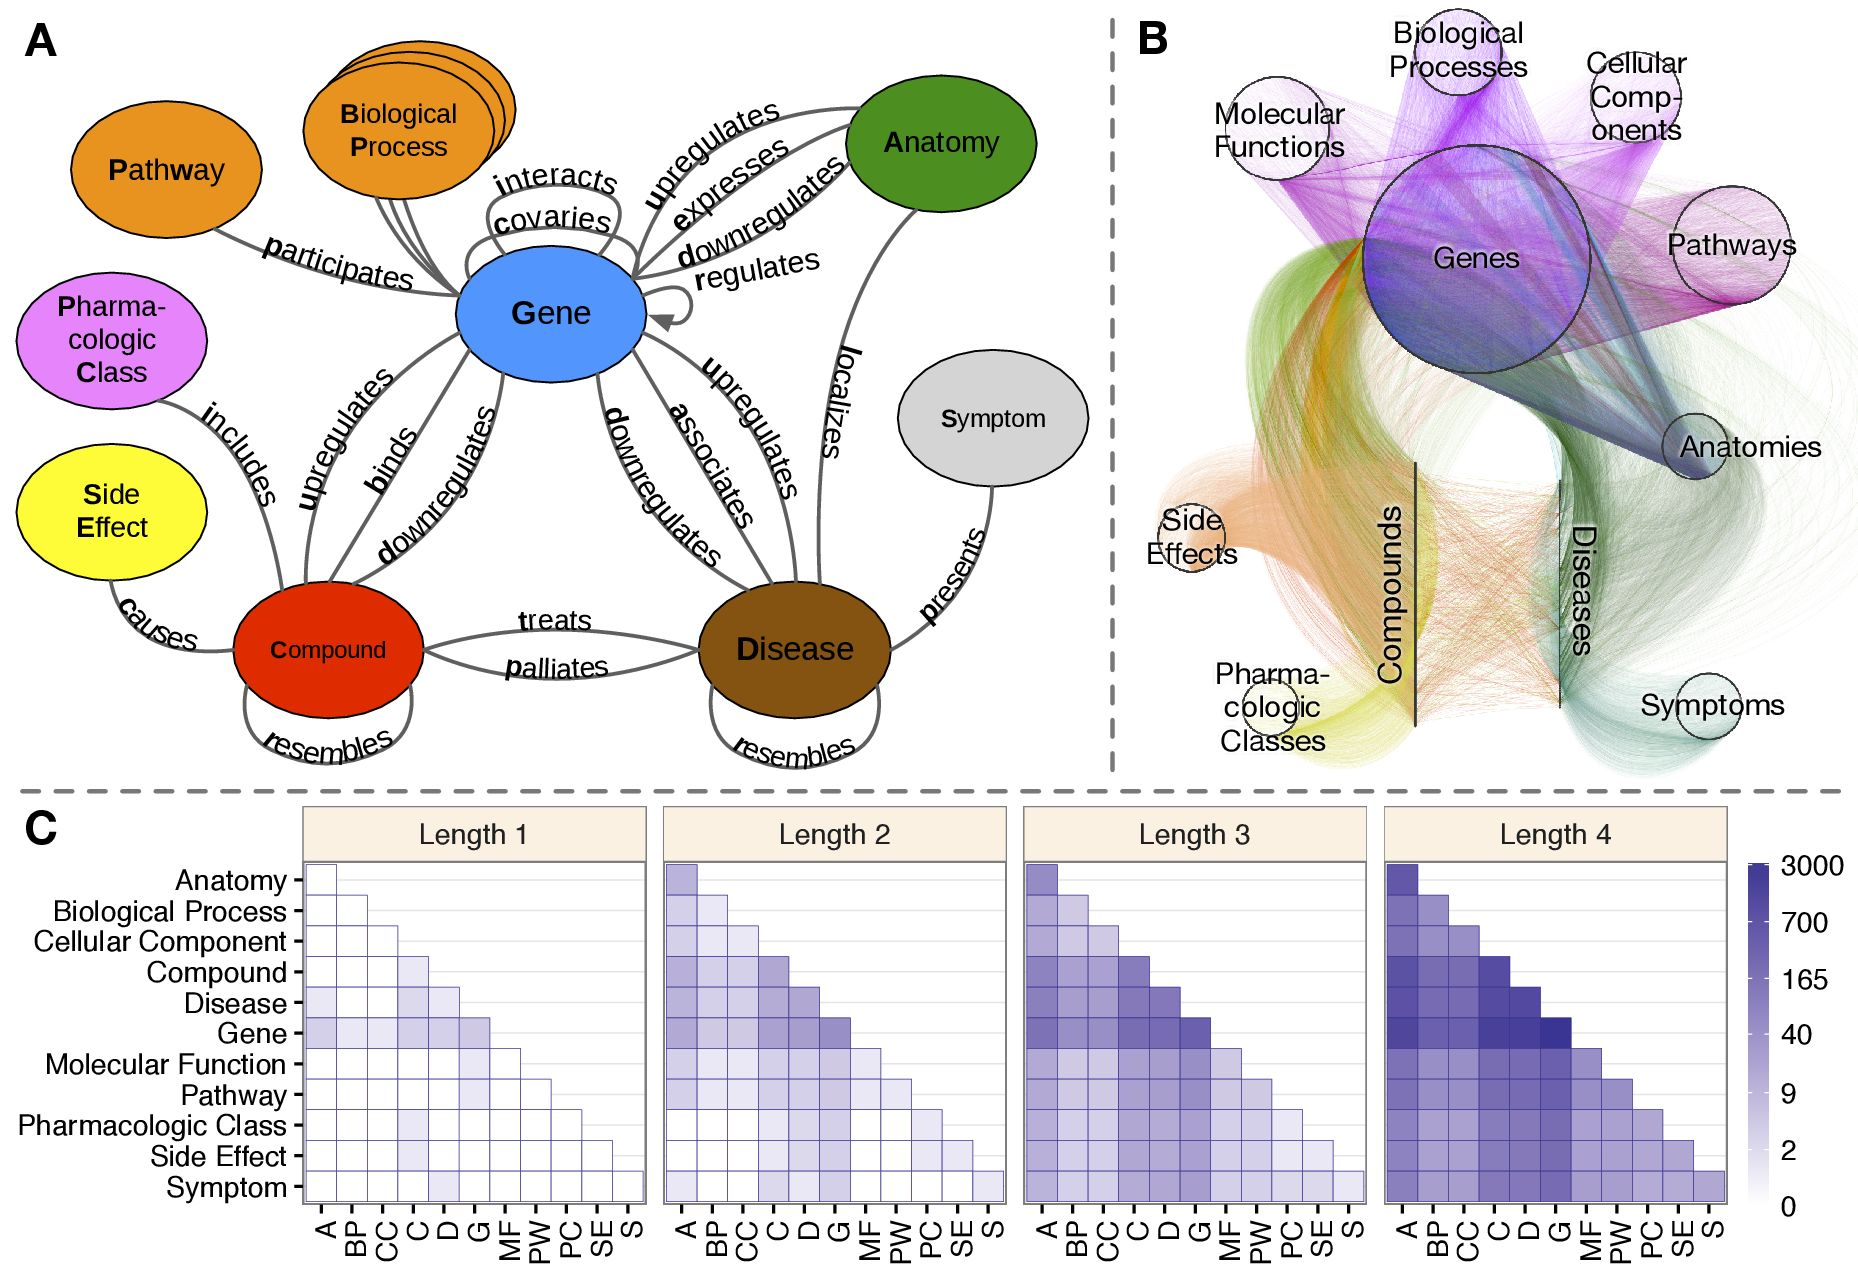
\includegraphics[width=\textwidth, height=0.45\textheight, keepaspectratio]{rysunki/elife-26726-fig1-v2.jpg}
    \caption{Hetionet knowledge graph}
    \label{fig:hetionet-original}
\end{figure}

%wstawić rysunek
%https://github.com/hetio/hetionet
%https://elifesciences.org/articles/26726/figures


\newpage % Rozdziały zaczynamy od nowej strony.
\section{Main Framework}

A causal knowledge graph is not merely a static record of the literature: it can be systematically audited, weighted, and enriched with observational data,
 and subsequently used as the basis for explainable clinical prediction of drug-related outcomes. This thesis operationalizes that idea through two 
 complementary graph neural network tasks, applied to a shared causal knowledge graph of pharmacotherapy:

 \begin{enumerate}[label=\alph*)]
    \item \textbf{Task A:} link prediction, which reconstructs and updates the knowledge graph based on real patient data;
    \item \textbf{Task B:} node classification, which predicts patient-specific clinical endpoints based on the knowledge graph and real patient data.
\end{enumerate}

Since both tasks operate on the same underlying knowledge graph, we adopt graph 
neural networks as the common modeling framework, and enrich them with 
Hierarchical Correlation Reconstruction (HCR). In Figure \ref{fig:architecture} there is presented 
a high-level approach to construct GNN with HCR. While the two tasks share this common foundation, their implementation details differ in several respects; 
we therefore present each task separately in the following subsections.
%moze tutaj damy referencje do Wide&Deep architecture - https://arxiv.org/abs/1606.07792


\begin{figure}[h]
    \centering
    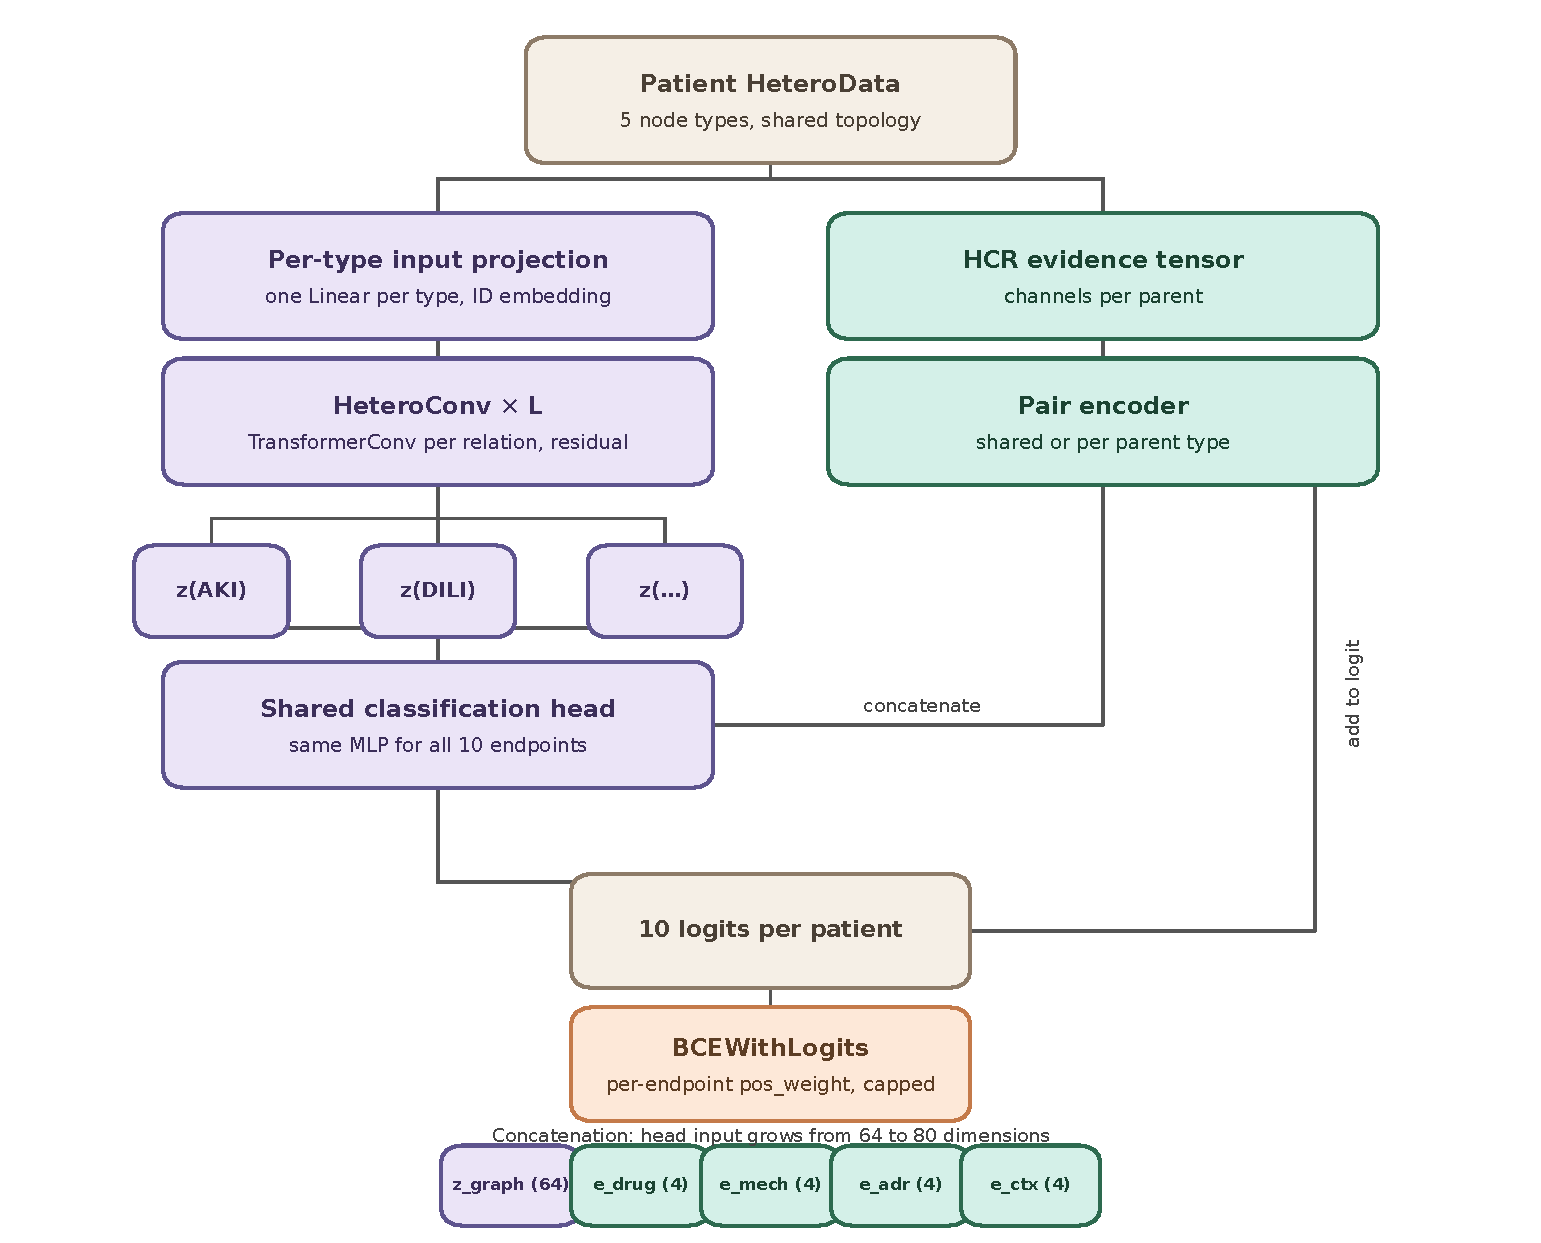
\includegraphics[width=0.95\textwidth,keepaspectratio]{rysunki/architecture_slide_multilabel_hcr.pdf}
    \caption{The presentation of approach to node classification task.}
    \label{fig:architecture}
\end{figure}

\subsection{Link prediction in Graph Reconstruction}


\subsection{Endpoint prediction}

Task B is formulated as multi-label node classification on a heterogeneous, per-patient graph. 
Rather than building one global graph and treating patients as additional nodes, every patient is represented 
as a copy of the same fixed causal DAG topology, with node feature vectors instantiated from that patient's 
individual covariates. The prediction targets are a fixed subset of clinical events on patient site. 
Formally, for a patient graph \(G_p = (V, E)\) shared across the cohort, with patient-specific node features
\(x_p\), the model computes

\[
\hat{y}_{p,e} = \sigma\big(f_\theta(G_p, x_p)_e\big), \quad e \in \mathcal{E}_{\text{target}}
\]

where \(f_\theta\) is a heterogeneous graph neural network shared across all patients, and only the leaf-level
target embeddings are read out by the classification head.

\subsubsection{Data Representation}

The first thing in applying GNNs is to built properly the input into neural network. The input graph for the node 
classification task was built based on: 

\begin{enumerate}[label=\alph*)]
    \item \textbf{nodes}
    \item \textbf{edges}
    \item \textbf{per-scenario patient sample table} 
\end{enumerate}

Based on those items \texttt{HeteroData} object was created which was represented by objects type presented in the table

\begin{table}[t]
    \centering
    \caption{Components of the per-patient \texttt{HeteroData} graph representation.}
    \label{tab:heterodata_components}
    \begin{tabularx}{\textwidth}{@{}l X@{}}
        \toprule
        \textbf{Component} & \textbf{Description} \\
        \midrule
        Node types &
        Six semantic categories of nodes shared across all patient graphs: \texttt{patient\_context}, \texttt{drug\_exposure}, \texttt{mechanism}, \texttt{adr\_or\_intermediate\_state}, \texttt{observation\_or\_selection}, and \texttt{clinical\_endpoint}. \\
        \addlinespace
        Relations &
        Keyed by \texttt{(src\_type, "to", dst\_type)} weighted by \texttt{edge\_attr} instead of using \texttt{edge\_type}. This keeps the number of distinct convolutional relation modules in \texttt{HeteroConv} small while still letting edge-type information reach the message function. \\
        \addlinespace
        Edge attributes (\texttt{edge\_attr}) &
        %signed effect size, activation frequency, mechanistic confidence, evidence weight, and the edge-type one-hot. Convolutions consuming a scalar \texttt{edge\_weight} (GraphConv/GCN) receive only the signed effect-size column; convolutions consuming a full \texttt{edge\_attr} (GAT, Transformer) receive the whole vector. \\
        Combination of \texttt{effect\_size} and \texttt{effect\_sign} \\
        \addlinespace
        Node features (\texttt{x}) &
        The patient's observed values for that node where the node. \\
        \bottomrule
    \end{tabularx}
\end{table}

The patient data is encoded on nodes level. In \cref{fig:architecture} there is presented the exemplary DAG for one 
of patient. 

\begin{figure}[h]
    \centering
    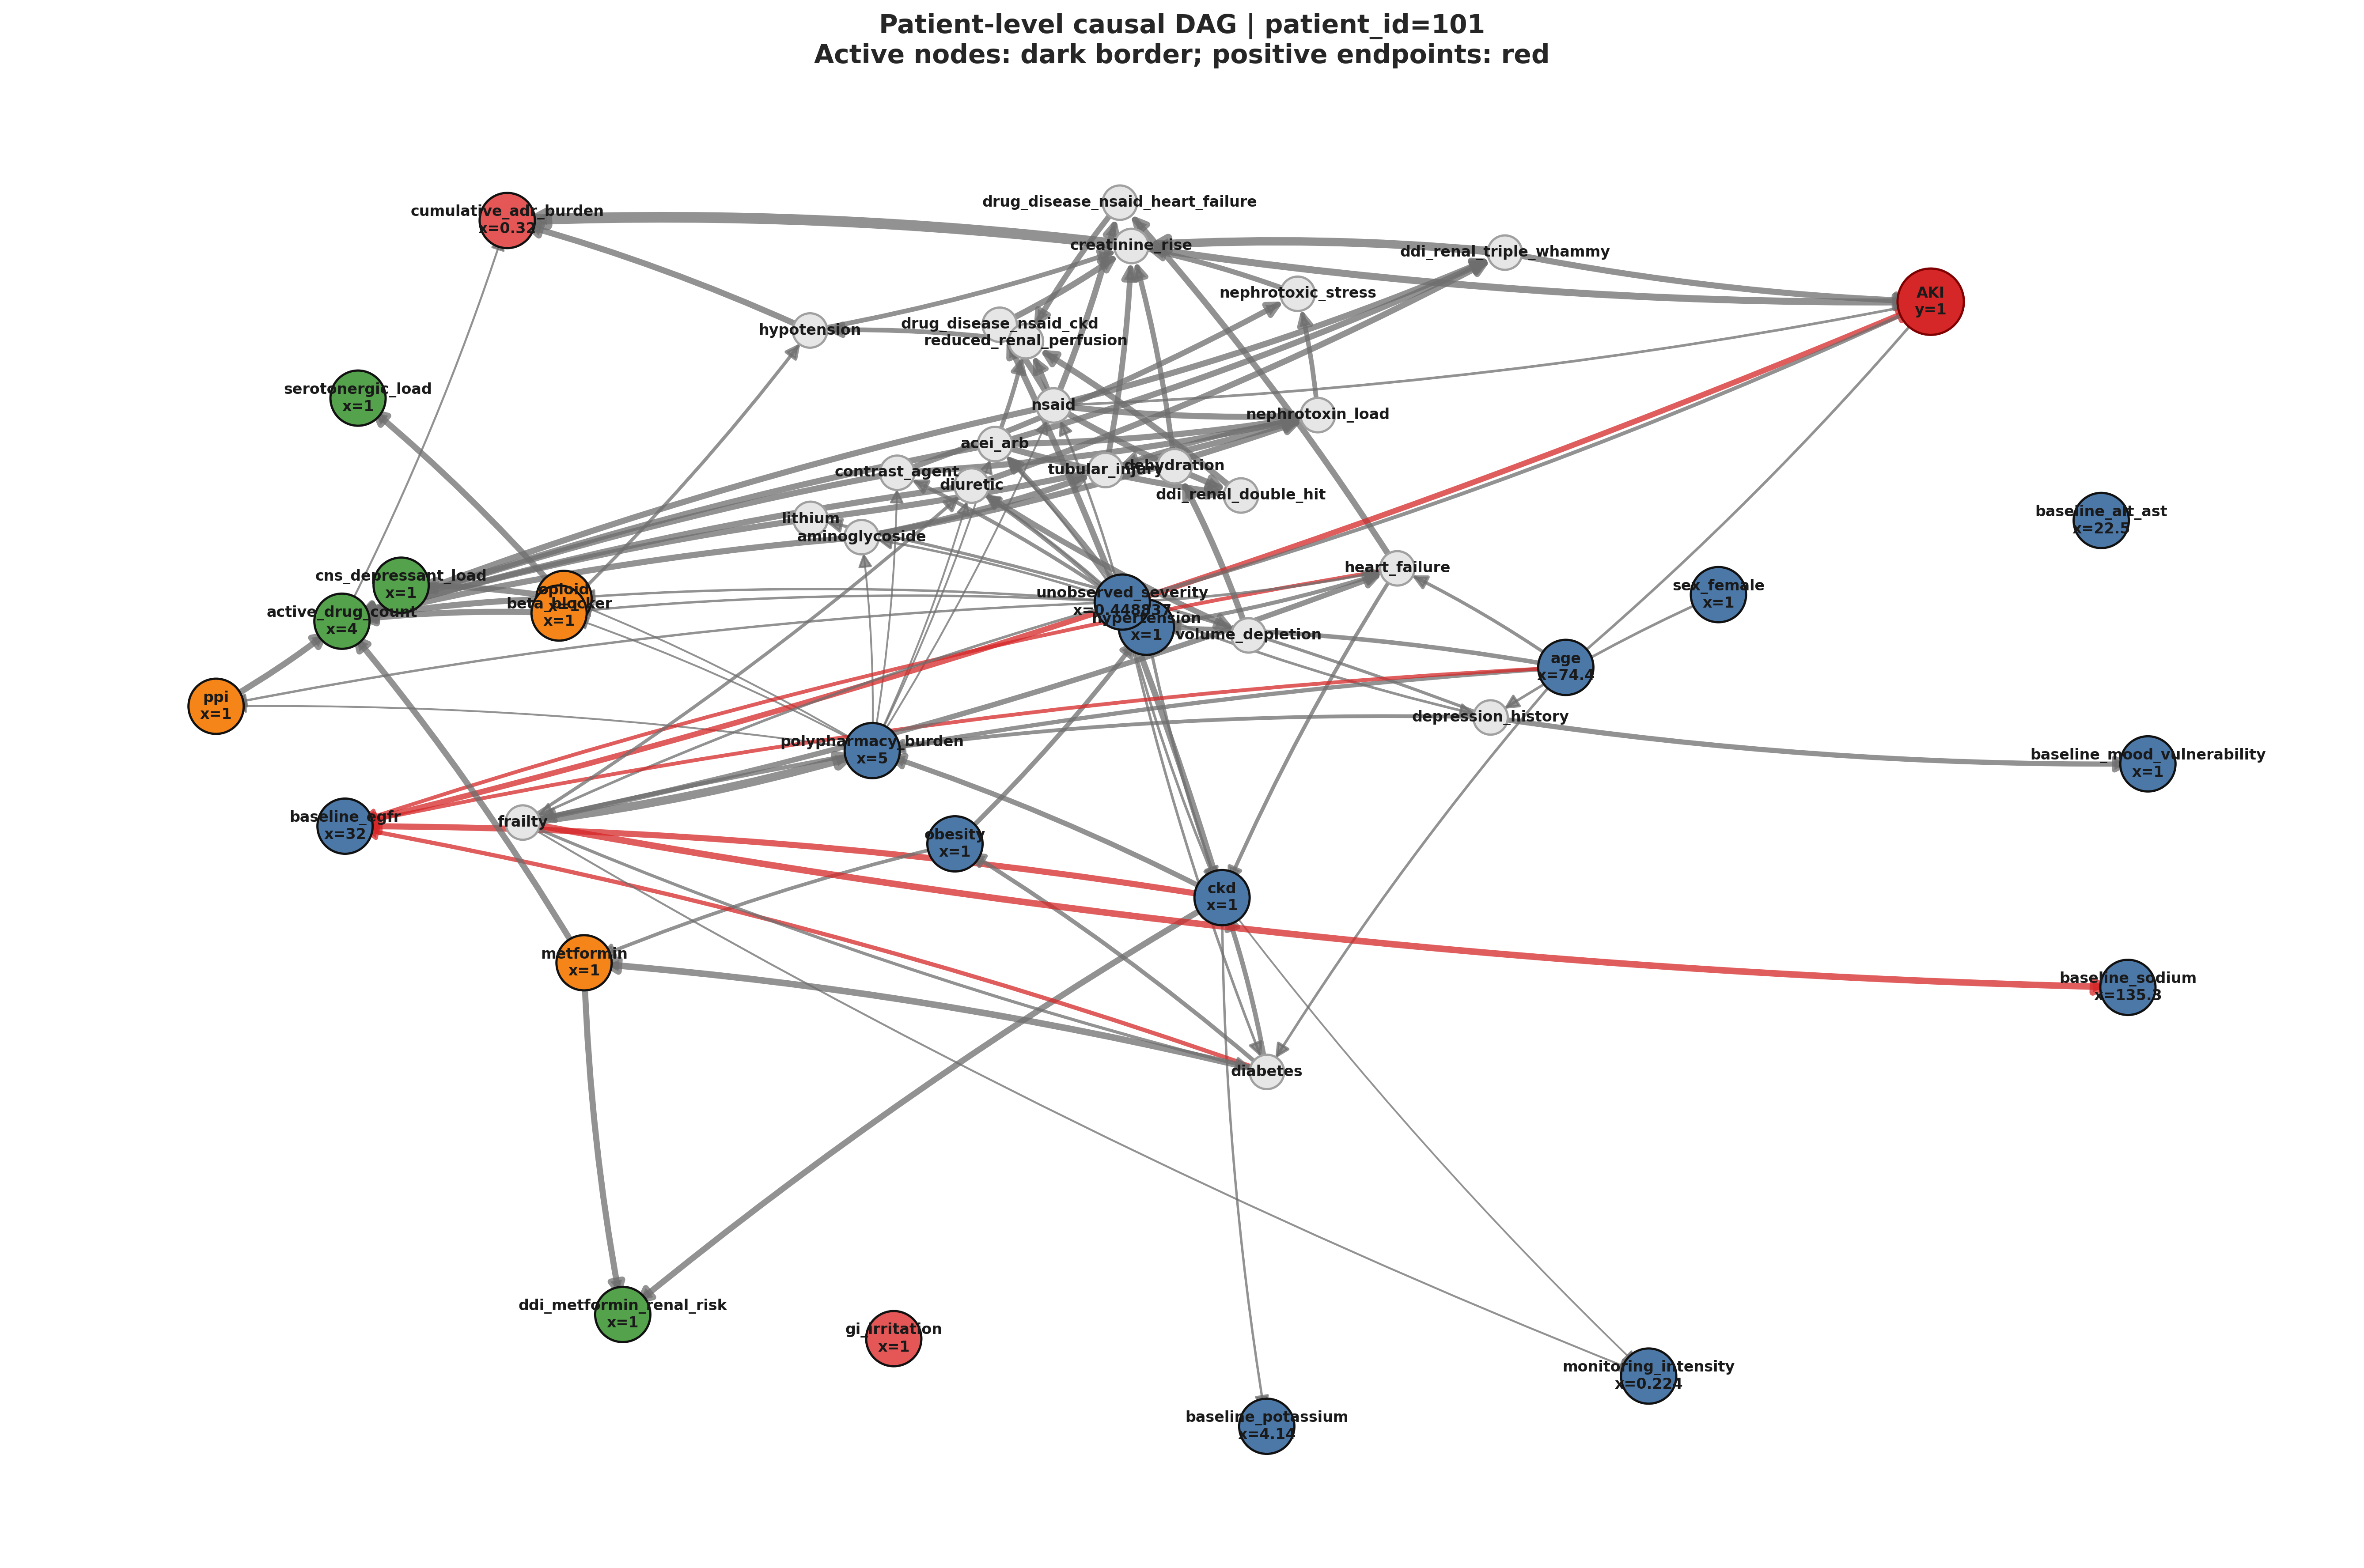
\includegraphics[width=\textwidth, height=0.45\textheight, keepaspectratio]{rysunki/patient_dag_101.png}
    \caption{The description of the two tasks addressed in the thesis.}
    \label{fig:patient_dag}
\end{figure}

Two structural exclusion mechanisms are applied before any feature is computed: 
\begin{enumerate}[label=\alph*)]
    \item nodes flagged \texttt{exclude\_from\_observed\_model} or \texttt{is\_latent} (hidden confounders); 
    \item nodes that are structural descendants of any endpoint in the DAG (e.g. documentation nodes such as 
    \texttt{hospital\_contact}, \texttt{fall\_reported}, which are caused by the endpoint rather than causal parents of it)
\end{enumerate}

 All normalization statistics (mean/std for continuous node values) 
 and all HCR evidence statistics (\cref{subsec:hcr_application}) are computed exclusively on the training split of patients, to 
 prevent both node-level and patient-level information leakage across splits.
 %trzeba dopisać wybor endpoints - dlaczego tak a nie inaczej
 %auc liczony bez endpoint Serotonin_syndrome Rhabdomyolysis Lactic_acidosis - bardzo rzadkich 

\subsubsection{Model architecture}

The core architecture is a stack of heterogeneous graph convolutional layers wrapped in \texttt{HeteroConv},
shared across relation types but parameterized identically for every patient graph. Four convolution backbones 
are supported through a common registry and were benchmarked against each other: GraphSAGE, and TransformerConv. 
As these operators were originally designed for homogeneous graphs,
each is instantiated once per edge type inside \texttt{HeteroConv}, so the heterogeneous DAG is handled without 
collapsing node/edge types into a single homogeneous graph.
As benefit of casual graph structure is possibility to encode deep structured path for node classification, 
multiple number of layers was tested to choose the best model.  
%root_weight

A design issue that was handled during experiments is the duplication of the self-transform across relations. 
Several PyG convolution layers (SAGEConv, TransformerConv) internally add their own linear self-loop term,
 wrapped per-relation inside \texttt{HeteroConv}, this term is silently duplicated once per incoming 
relation type for a given node type. The implementation removes this internal duplication 
(\texttt{root\_weight}=False for SAGE/Transformer) and replaces it with a single, explicit, 
controlled self-transform per layer per node type. 
% For GAT-family layers, where the self-dependency is baked into the attention query and cannot be disabled, the explicit self-transform 
% acts as an additional controlled term on top of the irreducible built-in dependency. GraphConv/GCN, which has no 
% \texttt{root\_weight} parameter at all, is deliberately excluded from this mechanism, since its built-in self-transform 
% cannot be removed without reimplementing the layer.
%node identity 

A node-identity embedding, added after the input projection, was introduced to resolve a specific representational 
collapse. Message-passing GNNs are bounded in expressive power by the 1-dimensional Weisfeiler-Lehman graph 
isomorphism test. In the dataset, several 
endpoint nodes of the same type (e.g. Serotonin syndrome, Rhabdomyolysis, Lactic acidosis) share 
identical static audited attributes (e.g. \texttt{severity\_weight}, observability) and comparable topological 
positions, and were therefore indistinguishable to the model except through such positional cues.
To break this symmetry, a learnable embedding table is maintained per node type, indexed by each node's fixed 
local index, and added to the projected input features before the first convolutional layer, following the same 
principle underlying position aware node embeddings in .
%oversmoothing (i will see if i should present it or rephrase it somehow)

This connects directly to the model's handling of oversmoothing. Using multiple message-passing layers risks oversmoothing 
the embedding signal, where repeated aggregation causes node representations to converge toward 
indistinguishability. To mitigate this, several oversmoothing countermeasures were applied: 
residual connections, Jumping Knowledge, DropEdge, and PairNorm. These methods were evaluated both 
individually and in combination with the HCR enrichment described in \cref{subsec:hcr_application}.

\subsubsection{HCR application}
\label{subsec:hcr_application}

In addition to the purely structural GNN pathway, approch presented in the thesis incorporates a statistical evidence 
side-channel - HCR described in details in \cref{subsec:hcr_def}. This channel is motivated by the 
observation that some parent-endpoint dependencies are well captured by simple, well-understood pairwise 
statistics computed directly from the training cohort, and that combining such statistics with the deep GNN 
representation captures the strong signal from direct parents and smoothed signal from further layers.
There were run couple of experiments with HCR configurations and GNNs. However, in general the approach was about
computation of contingency-table statistics for each target endpoint and direct parents or pre-direct parents in 
the audited DAG (restricted to nodes with inferred 
binary, count, or continuous value types). The statistics computed was as followed per (parent, endpoint) 
pair: the \(\varphi\)-coefficient, normalized mutual information, a tanh-scaled log odds 
ratio, risk difference, and a tanh-scaled log lift, plus prevalence and support terms. There are nine to forty-one 
channels depending on configuration.
%dopisac dlaczego u nas jest 41/42 a w przypadku task a 41
%leave-one-out

As these coefficients are computed with the patient's own endpoint label as part of the statistic, a naive 
computation would leak the label into the feature. This was addressed with an 
exact leave-one-out correction: every training patient's coefficient is computed from all other training patients
only, using a closed-form re-weighting of the population statistic.
 
 Continuous and count-valued parents are mapped to comparable pseudo-uniform scores via a train-only empirical 
 CDF transform (with deterministic, patient-ID-seeded jitter for count variables), and Legendre polynomial bases 
 are used to capture non-linear dependence on continuous parents.

 Three integration modes were supported: 
 \begin{enumerate}[label=\alph*)]
    \item linear approach - a single scalar HCR score added directly to the GNN logit,
    \item nonlinear encoder - parent-endpoint evidence vectors pooled and passed through a shared MLP
    \item separate encoders per parent node type - every direct parent passed through a separated MLP
    \item triple relations - relations not only focused on direct parents, but direct parents and grandparents. 
 \end{enumerate}


 The pooling in HCRPairEncoder masks out padding positions (endpoints with fewer parents than the batch's 
 maximum) and returns a neutral zero vector for endpoints with no eligible parents, avoiding division by zero.

%jak jest wszystko polaczone dokladniej


\subsubsection{Training setup}

Training iterates over patient graphs batched via PyG DataLoader. The experiments were run with
targeted binary cross-entropy and focal loss with class-balance-aware weighting. 
Weight and focal alpha were computed from the training split's endpoint prevalence, since clinical outcomes
are rare and highly imbalanced. Model selection uses ReduceLROnPlateau on validation performance, and 
evaluation is reported separately per endpoint and in aggregate, using AUROC, AUPRC, and prevalence-normalized 
lift.
%alongside the representation-level over-smoothing diagnostics (MAD, cosine similarity, Dirichlet energy) 
%used to relate architectural choices. 
 As the synthetic dataset generated for this project contains
 rare events and class imbalance, AUPRC was chosen as a key performance
 metric. It focuses on the positive class and reflects the trade-off
 between precision and recall. Below there are included the equations for calculating metrics.
 
 \emph{AUC} is the area under the receiver operating characteristic curve (ROC-AUC) 
 and is defined as:
 \begin{equation}
   \mathrm{ROC\mbox{-}AUC}
   =
   \int_0^1 \mathrm{TPR}(\mathrm{FPR})\,d\mathrm{FPR}.
   \end{equation}
   where $\mathrm{TPR}$ is the true positive rate and $\mathrm{FPR}$ is the false positive rate.
 
 \emph{AUPRC} is the area under the precision--recall curve and is defined as:
 \begin{equation}
   \mathrm{AP} =
   \sum_{n}
   \left(R_n - R_{n-1}\right) P_n,
   \end{equation}
   where $P_n$ and $R_n$ denote precision and recall at the $n$-th threshold,
   respectively.
 
 \emph{Lift} is the AUPRC divided by the prevalence baseline, that is, the
 factor by which the model improves over a random ranking, e.g. at a mean
 prevalence of $5.5\%$ a lift of $2.3$ corresponds to an AUPRC of $0.125$.
 
 In addition to the traditional metrics described above, an oracle AUC was
 calculated for the node-classification task.
 As the dataset for this task is synthetic,
 the exact function used to generate each endpoint is known, which allows to calculate AUC oracle.
 In the final assesement of the models we compared the AUC and AUC oracle 
 (\%ceiling) with the following formula:
 
 \begin{equation}
   \frac{\mathrm{AUC} - 0.5}{\mathrm{AUC}_{\mathrm{Oracle}} - 0.5} \cdot 100\%,
   \label{eq:pct-ceiling}
 \end{equation}
 %
 where $\mathrm{AUC}_{\mathrm{Oracle}} = 0.651$ is the AUC oracle averaged
 over the same eight endpoints. This metric expresses the
 share of attainable signal recovered by the model. The model increased performance
 is calculated from random baseline model performance which is 0.5.
 
 
 
\newpage % Rozdziały zaczynamy od nowej strony.
\section{Experiments results}





\subsection{Link prediction in graph reconstuction}


\subsubsection{Synthethic dataset}


\subsubsection{Proxy dataset}


\subsection{Endpoint prediction}

The first aim of experiments was to choose the best architecture for the problem. The following architecture was tested RGCN, SAGE, Transformer. 
All of architecture is designed for homogenous graphs. As pharmaceutical data that we used was structured in heterogenous graph, all of architecture was implemented in heterogenous convolutional layer - heteroconv.  

\subsubsection{Synthethic dataset}

The results for the presented experiments are following. 

\begin{table}[htbp]
  \centering
  \scriptsize
  \caption{Transformers with HCR and residual}
  \setlength{\tabcolsep}{2.5pt}
  \label{tab:bayes-hcr-jk}
  \begin{tabular}{clllcccccccc}
  \toprule
   &  &  &  & \multicolumn{4}{c}{Validation} & \multicolumn{4}{c}{Test} \\
  \cmidrule(lr){5-8}\cmidrule(lr){9-12}
  $L$ & Residual & HCR & JK & AUC & AUPRC & Lift & \%AUC & AUC & AUPRC & Lift & \%AUC \\
  \midrule
  1 & no & --- & --- & 0.621 & 0.1252 & 2.30 & 80 & 0.618 & 0.1192 & 2.19 & 78 \\
  \addlinespace[4pt]
  3 & no & --- & --- & 0.546 & 0.0850 & 1.56 & 30 & 0.550 & 0.0752 & 1.38 & 33 \\
  3 & no & --- & cat & 0.606 & 0.1383 & 2.54 & 71 & 0.615 & 0.1235 & 2.27 & 76 \\
  3 & no & linear 41D & --- & 0.599 & 0.1214 & 2.23 & 66 & 0.610 & 0.1066 & 1.96 & 73 \\
  3 & no & linear 41D & cat & 0.608 & 0.1379 & 2.53 & 72 & 0.616 & 0.1246 & 2.29 & 77 \\
  3 & yes & --- & --- & 0.624 & 0.1353 & 2.48 & 82 & 0.618 & 0.1221 & 2.24 & 78 \\
  3 & yes & --- & cat & 0.624 & 0.1357 & 2.49 & 82 & 0.620 & 0.1236 & 2.27 & 80 \\
  3 & yes & linear 41D & cat & \textbf{0.629} & 0.1336 & 2.45 & \textbf{85} & 0.620 & 0.1243 & 2.28 & 80 \\
  3 & yes & nonlin. 41D & --- & 0.622 & 0.1347 & 2.47 & 81 & 0.622 & 0.1231 & 2.26 & 81 \\
  3 & yes & nonlin. bin. & --- & 0.624 & 0.1348 & 2.47 & 82 & 0.622 & 0.1229 & 2.26 & 81 \\
  3 & yes & typed 41D & --- & 0.619 & 0.1342 & 2.47 & 79 & 0.611 & 0.1211 & 2.22 & 74 \\
  \addlinespace[4pt]
  6 & no & --- & --- & 0.526 & 0.0671 & 1.23 & 17 & 0.524 & 0.0635 & 1.17 & 16 \\
  6 & no & --- & cat & 0.617 & \textbf{0.1415} & \textbf{2.60} & 78 & 0.621 & \textbf{0.1285} & \textbf{2.36} & 80 \\
  6 & no & linear 41D & --- & 0.616 & 0.1206 & 2.21 & 77 & 0.608 & 0.1104 & 2.03 & 72 \\
  6 & no & linear 41D & cat & 0.615 & 0.1409 & 2.59 & 77 & 0.623 & 0.1272 & 2.34 & 82 \\
  6 & yes & --- & --- & 0.624 & 0.1359 & 2.50 & 82 & 0.621 & 0.1225 & 2.25 & 80 \\
  6 & yes & --- & cat & 0.624 & 0.1352 & 2.48 & 82 & 0.622 & 0.1239 & 2.28 & 81 \\
  6 & yes & linear 41D & cat & 0.626 & 0.1360 & 2.50 & 83 & \textbf{0.628} & 0.1251 & 2.30 & \textbf{85} \\
  6 & yes & nonlin. 41D & --- & 0.620 & 0.1325 & 2.43 & 80 & 0.615 & 0.1208 & 2.22 & 76 \\
  6 & yes & nonlin. bin. & --- & 0.604 & 0.1179 & 2.16 & 69 & 0.604 & 0.1078 & 1.98 & 69 \\
  6 & yes & typed 41D & --- & 0.621 & 0.1338 & 2.46 & 80 & 0.617 & 0.1230 & 2.26 & 78 \\
  \bottomrule
  \end{tabular}
  \end{table}
  
  \begin{table}[htbp]
  \centering
  \scriptsize
  \caption{Transformers with oversmoothing methods applied}
  \setlength{\tabcolsep}{2.5pt}
  \label{tab:bayes-antiovs}
  \begin{tabular}{cllcccccccc}
  \toprule
   &  &  & \multicolumn{4}{c}{Validation} & \multicolumn{4}{c}{Test} \\
  \cmidrule(lr){4-7}\cmidrule(lr){8-11}
  $L$ & Residual & Method & AUC & AUPRC & Lift & \%AUC & AUC & AUPRC & Lift & \%AUC \\
  \midrule
  1 & no & --- & 0.621 & 0.1252 & 2.30 & 80 & 0.618 & 0.1192 & 2.19 & 78 \\
  \addlinespace[4pt]
  3 & no & --- & 0.546 & 0.0850 & 1.56 & 30 & 0.550 & 0.0752 & 1.38 & 33 \\
  3 & no & JK cat & 0.606 & 0.1383 & 2.54 & 71 & 0.615 & 0.1235 & 2.27 & 76 \\
  3 & no & JK max & 0.622 & 0.1372 & 2.52 & 81 & 0.619 & 0.1240 & 2.28 & 79 \\
  3 & no & DropEdge & 0.546 & 0.0800 & 1.47 & 30 & 0.547 & 0.0726 & 1.33 & 31 \\
  3 & no & JK cat + DropEdge & 0.623 & 0.1386 & 2.55 & 81 & 0.623 & 0.1249 & 2.30 & 82 \\
  3 & no & JK max + DropEdge & 0.626 & 0.1389 & 2.55 & 84 & 0.622 & 0.1219 & 2.24 & 81 \\
  3 & yes & --- & 0.624 & 0.1353 & 2.48 & 82 & 0.618 & 0.1221 & 2.24 & 78 \\
  3 & yes & JK cat & 0.624 & 0.1357 & 2.49 & 82 & 0.620 & 0.1236 & 2.27 & 80 \\
  3 & yes & JK max & 0.626 & 0.1370 & 2.52 & 83 & 0.620 & 0.1234 & 2.27 & 79 \\
  3 & yes & DropEdge & 0.626 & 0.1341 & 2.46 & 84 & 0.622 & 0.1237 & 2.27 & 81 \\
  3 & yes & JK cat + DropEdge & \textbf{0.629} & 0.1362 & 2.50 & \textbf{85} & \textbf{0.624} & 0.1248 & 2.29 & \textbf{83} \\
  3 & yes & JK max + DropEdge & 0.625 & 0.1359 & 2.50 & 83 & 0.622 & 0.1238 & 2.28 & 81 \\
  \addlinespace[4pt]
  6 & no & --- & 0.526 & 0.0671 & 1.23 & 17 & 0.524 & 0.0635 & 1.17 & 16 \\
  6 & no & JK cat & 0.617 & \textbf{0.1415} & \textbf{2.60} & 78 & 0.621 & \textbf{0.1285} & \textbf{2.36} & 80 \\
  6 & yes & --- & 0.624 & 0.1359 & 2.50 & 82 & 0.621 & 0.1225 & 2.25 & 80 \\
  6 & yes & JK cat & 0.624 & 0.1352 & 2.48 & 82 & 0.622 & 0.1239 & 2.28 & 81 \\
  \bottomrule
  \end{tabular}
  \end{table}

  \begin{table}[htbp]
    \centering
    \footnotesize
    \caption{Oversmoothing metrics}
    \label{tab:ovs-antiovs}
    \begin{tabular}{cllccccccc}
    \toprule
    $L$ & Residual & Metoda & MAD & CosSim & Rank & DirE & Std & $E_L/E_0$ & $\mathrm{MAD}_L/\mathrm{MAD}_0$ \\
    \midrule
    1 & no & --- & 0.882 & 0.571 & 0.229 & 0.178 & 0.168 & 0.115 & 1.585 \\
    \addlinespace[4pt]
    3 & no & --- & 0.799 & 0.630 & 0.125 & 0.041 & 0.083 & 0.057 & 0.898 \\
    3 & no & JK cat & 0.837 & 0.603 & 0.070 & 0.098 & 0.088 & 0.018 & 1.138 \\
    3 & no & JK max & 0.766 & 0.669 & 0.208 & 0.271 & 0.197 & 0.019 & 1.088 \\
    3 & no & DropEdge & 0.750 & 0.652 & 0.135 & 0.053 & 0.086 & 0.042 & 0.871 \\
    3 & no & JK cat + DropEdge & 0.827 & 0.610 & 0.073 & 0.073 & 0.082 & 0.020 & 1.093 \\
    3 & no & JK max + DropEdge & 0.727 & 0.687 & 0.190 & 0.175 & 0.153 & 0.024 & 1.161 \\
    3 & yes & --- & 0.774 & 0.689 & 0.180 & 0.189 & 0.182 & 0.098 & 1.112 \\
    3 & yes & JK cat & 0.826 & 0.630 & 0.104 & 0.219 & 0.174 & 0.038 & 1.024 \\
    3 & yes & JK max & 0.630 & 0.816 & 0.315 & 0.337 & 0.219 & 0.059 & 1.039 \\
    3 & yes & DropEdge & 0.784 & 0.682 & 0.169 & 0.110 & 0.143 & 0.102 & 1.102 \\
    3 & yes & JK cat + DropEdge & 0.826 & 0.633 & 0.099 & 0.215 & 0.177 & 0.047 & 0.984 \\
    3 & yes & JK max + DropEdge & 0.678 & 0.799 & 0.271 & 0.279 & 0.206 & 0.066 & 1.094 \\
    \addlinespace[4pt]
    6 & no & --- & 0.808 & 0.634 & 0.125 & 0.049 & 0.094 & 0.080 & 0.781 \\
    6 & no & JK cat & 0.813 & 0.611 & 0.037 & 0.053 & 0.056 & 0.012 & 1.068 \\
    6 & yes & --- & 0.756 & 0.702 & 0.133 & 0.096 & 0.135 & 0.056 & 1.055 \\
    6 & yes & JK cat & 0.823 & 0.652 & 0.056 & 0.163 & 0.127 & 0.017 & 0.939 \\
    \bottomrule
    \end{tabular}
    \end{table}


\subsubsection{Proxy dataset}


% =====================================================================
%  PROXY DATASET RESULTS (Hetionet, cut A, proxy3_clean)
%  1552 compounds, 20 endpoints, seed 42, conv_type = transformer,
%  hidden = 64, batch = 8, lr = 1e-3, dropedge = 0.0
%  Jumping knowledge: NOT used in any configuration.
%
%  PREAMBLE:
%    \usepackage{booktabs}
%    \usepackage{siunitx}
%    \sisetup{detect-all, table-number-alignment=center}
%
%  Epoch selected on the validation set; test metrics recorded at the
%  end of training.
% =====================================================================


% ---------------------------------------------------------------------
% TABLE 1 - full observability regime
% ---------------------------------------------------------------------
\begin{table}[H]
  \centering
  \caption{Results under full observability on the proxy dataset. The
    epoch was selected on the validation set. \texttt{---} in the HCR
    column denotes a model without the HCR branch. Lift is AUPRC
    divided by the prevalence baseline. Jumping knowledge was not used
    in any configuration.}
  \label{tab:proxy-full}
  \sisetup{table-format=1.3}
  \begin{tabular}{ccl SSS SSS}
    \toprule
    & & & \multicolumn{3}{c}{Validation} & \multicolumn{3}{c}{Test} \\
    \cmidrule(lr){4-6}\cmidrule(lr){7-9}
    $L$ & Residual & HCR & {AUC} & {AUPRC} & {Lift} & {AUC} & {AUPRC} & {Lift} \\
    \midrule
    1 & no  & ---            & 0.757 & 0.188 & 7.92  & 0.664 & 0.120 & 6.49 \\
    1 & no  & nonlin.\ 9D    & 0.763 & 0.207 & 8.75  & 0.657 & 0.120 & 6.47 \\
    1 & no  & typed 41D      & 0.759 & 0.194 & 8.17  & 0.663 & 0.116 & 6.29 \\
    \addlinespace[2pt]
    1 & yes & ---            & 0.756 & 0.196 & 8.26  & 0.669 & 0.106 & 5.72 \\
    1 & yes & nonlin.\ 9D    & 0.756 & 0.201 & 8.49  & 0.670 & 0.135 & 7.31 \\
    1 & yes & typed 41D      & 0.754 & 0.185 & 7.79  & 0.671 & 0.124 & 6.71 \\
    \midrule
    3 & no  & ---            & 0.756 & 0.199 & 8.38  & {\bfseries 0.722} & 0.152 & 8.24 \\
    3 & no  & nonlin.\ 9D    & 0.805 & 0.275 & 11.62 & 0.686 & 0.169 & 9.14 \\
    3 & no  & typed 41D      & 0.812 & 0.243 & 10.26 & 0.678 & 0.154 & 8.32 \\
    \addlinespace[2pt]
    3 & yes & ---            & 0.799 & 0.225 & 9.48  & 0.685 & 0.166 & 8.97 \\
    3 & yes & nonlin.\ 9D    & 0.814 & 0.235 & 9.90  & 0.714 & 0.183 & 9.92 \\
    3 & yes & typed 41D      & 0.802 & 0.255 & 10.76 & 0.678 & 0.151 & 8.16 \\
    \midrule
    6 & no  & ---            & 0.610 & 0.121 & 5.11  & 0.585 & 0.077 & 4.14 \\
    6 & no  & nonlin.\ 9D    & 0.782 & 0.210 & 8.86  & 0.680 & 0.174 & 9.42 \\
    6 & no  & typed 41D      & 0.794 & 0.235 & 9.89  & 0.680 & 0.126 & 6.84 \\
    \addlinespace[2pt]
    6 & yes & ---            & 0.817 & 0.255 & 10.77 & 0.728 & 0.173 & 9.36 \\
    6 & yes & nonlin.\ 9D    & {\bfseries 0.832} & {\bfseries 0.310} & {\bfseries 13.06} & {\bfseries 0.760} & 0.179 & 9.70 \\
    6 & yes & typed 41D      & 0.815 & 0.284 & 11.99 & 0.744 & {\bfseries 0.239} & {\bfseries 12.91} \\
    \bottomrule
  \end{tabular}
\end{table}


% ---------------------------------------------------------------------
% TABLE 2 - bedside observability regime
% ---------------------------------------------------------------------
\begin{table}[H]
  \centering
  \caption{Results under restricted (\emph{bedside}) observability,
    $L=3$.}
  \label{tab:proxy-bedside}
  \sisetup{table-format=1.3}
  \begin{tabular}{cl SS SSS}
    \toprule
    & & \multicolumn{2}{c}{Validation} & \multicolumn{3}{c}{Test} \\
    \cmidrule(lr){3-4}\cmidrule(lr){5-7}
    Residual & HCR & {AUC} & {Lift} & {AUC} & {AUPRC} & {Lift} \\
    \midrule
    no  & ---             & 0.568 & 4.20  & 0.556 & 0.062 & 3.36 \\
    no  & lin.\ 41D       & 0.730 & 10.09 & 0.681 & 0.150 & 8.10 \\
    no  & nonlin.\ 41D    & 0.751 & 9.39  & 0.678 & 0.154 & 8.35 \\
    no  & typed 41D       & 0.753 & 9.45  & 0.679 & 0.135 & 7.31 \\
    \addlinespace[2pt]
    yes & ---             & 0.568 & 4.39  & 0.555 & 0.076 & 4.14 \\
    yes & lin.\ 41D       & 0.732 & 10.78 & 0.683 & 0.168 & 9.10 \\
    yes & nonlin.\ 41D    & 0.754 & 10.24 & 0.679 & 0.164 & 8.89 \\
    yes & typed 41D       & 0.754 & 10.18 & 0.678 & 0.173 & 9.33 \\
    \bottomrule
  \end{tabular}
\end{table}


% ---------------------------------------------------------------------
% TABLE 3 - representation smoothing metrics
% ---------------------------------------------------------------------
\begin{table}[H]
  \centering
  \caption{Representation smoothing metrics under full observability,
    measured on the validation set. By the conventional reading, lower
    MAD and higher cosine similarity indicate stronger smoothing.
    Validation AUC is repeated for comparison. Note that residual
    configurations appear more smoothed by every metric while
    performing better.}
  \label{tab:proxy-oversmoothing}
  \sisetup{table-format=1.4}
  \begin{tabular}{ccl SSSS S[table-format=1.3]}
    \toprule
    $L$ & Residual & HCR & {MAD} & {Cos.\ sim.} & {Cos.\ sim.\ (ep.)} & {Dirichlet} & {AUC} \\
    \midrule
    1 & no  & ---         & 0.7691 & 0.6216 & 0.8246 & 0.2706 & 0.757 \\
    1 & no  & nonlin.\ 9D & 0.7629 & 0.6142 & 0.7844 & 0.2495 & 0.763 \\
    1 & no  & typed 41D   & 0.7684 & 0.6191 & 0.8148 & 0.2706 & 0.759 \\
    \addlinespace[2pt]
    1 & yes & ---         & 0.7363 & 0.7042 & 0.7606 & 0.5724 & 0.756 \\
    1 & yes & nonlin.\ 9D & 0.7448 & 0.6946 & 0.7060 & 0.5048 & 0.756 \\
    1 & yes & typed 41D   & 0.7410 & 0.7026 & 0.7899 & 0.5022 & 0.754 \\
    \midrule
    3 & no  & ---         & 0.6515 & 0.6798 & 0.9582 & 0.1175 & 0.756 \\
    3 & no  & nonlin.\ 9D & 0.7067 & 0.6641 & 0.8365 & 0.0904 & 0.805 \\
    3 & no  & typed 41D   & 0.7235 & 0.6314 & 0.7333 & 0.0972 & 0.812 \\
    \addlinespace[2pt]
    3 & yes & ---         & 0.4842 & 0.8319 & 0.7772 & 0.3712 & 0.799 \\
    3 & yes & nonlin.\ 9D & 0.5517 & 0.7782 & 0.7752 & 0.3905 & 0.814 \\
    3 & yes & typed 41D   & 0.5113 & 0.8275 & 0.7132 & 0.4044 & 0.802 \\
    \midrule
    6 & no  & ---         & 0.7060 & 0.6530 & 0.8604 & 0.1024 & 0.610 \\
    6 & no  & nonlin.\ 9D & 0.7101 & 0.6495 & 0.7815 & 0.0892 & 0.782 \\
    6 & no  & typed 41D   & 0.7222 & 0.6408 & 0.8657 & 0.0949 & 0.794 \\
    \addlinespace[2pt]
    6 & yes & ---         & 0.5634 & 0.7975 & 0.7949 & 0.3143 & 0.817 \\
    6 & yes & nonlin.\ 9D & 0.5030 & 0.8174 & 0.6658 & 0.2636 & 0.832 \\
    6 & yes & typed 41D   & 0.5623 & 0.8095 & 0.8472 & 0.3930 & 0.815 \\
    \bottomrule
  \end{tabular}
\end{table}
\newpage % Rozdziały zaczynamy od nowej strony.
\section{Models benchmark}

results for proxy dataset



\newpage % Rozdziały zaczynamy od nowej strony.
\subsection{Link prediction}




\newpage % Rozdziały zaczynamy od nowej strony.
\subsection{Hetionet knowledge graph}
\label{subsec:benchmark-endpoint}

Task~B is evaluated on a benchmark dataset derived from Hetionet. 
Hetionet is a heterogeneous network
(\emph{hetnet}) that integrates biomedical knowledge from 29 publicly
available resources. It represents biological and pharmacological entities
as nodes and documented relationships between them as typed edges.

Hetionet v1.0 contains 47{,}031 nodes belonging to 11 node types and
2{,}250{,}197 relationships of 24 types. The graph includes compounds,
diseases, genes, anatomies, pathways, biological processes, molecular
functions, cellular components, pharmacologic classes, side effects, and
symptoms. This heterogeneous structure makes Hetionet suitable for node classification task described further. 
The details of benchmark check are included in Section ~\ref{subsec:benchmark-endpoint}.

\begin{figure}[h]
    \centering
    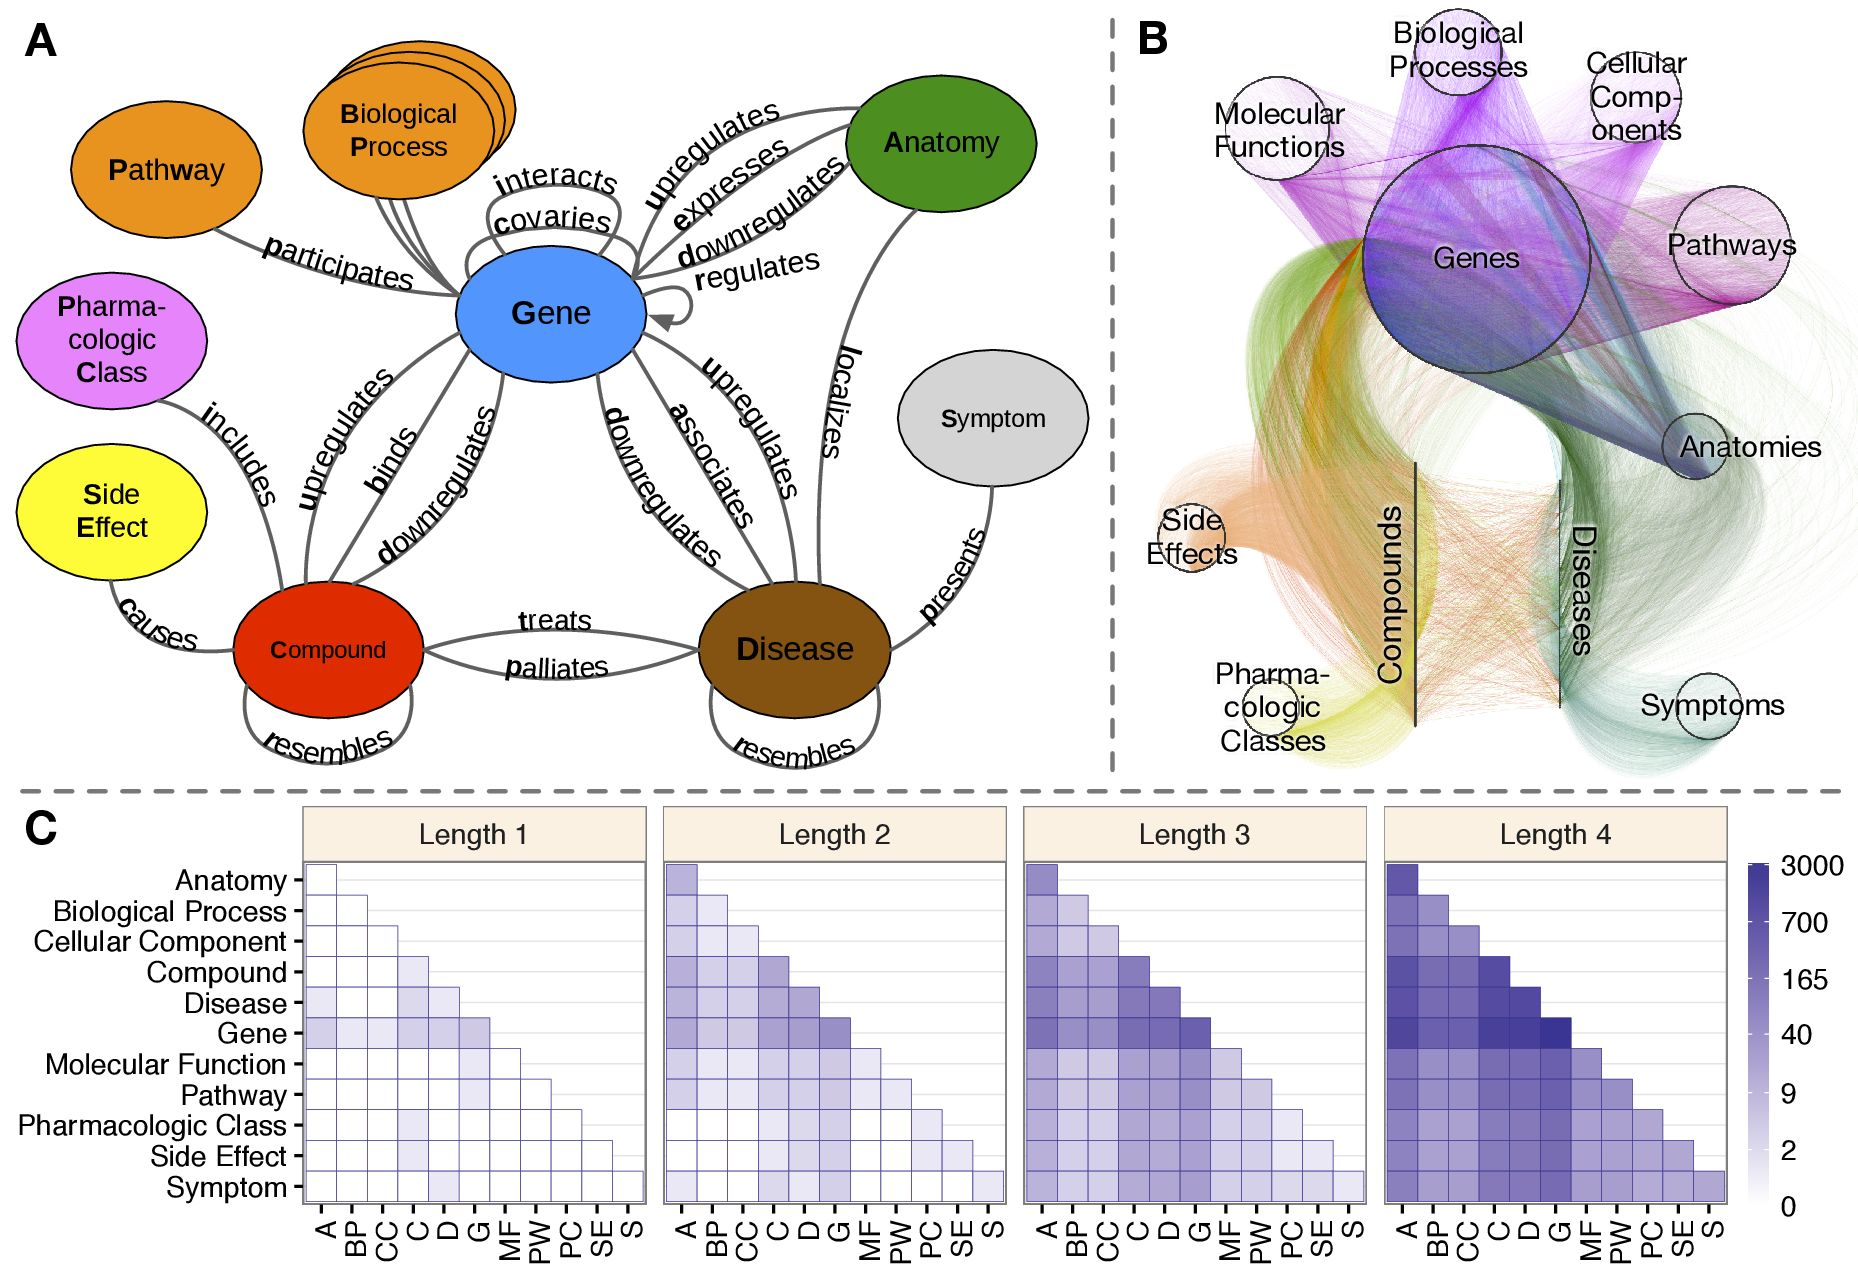
\includegraphics[width=\textwidth, height=0.45\textheight, keepaspectratio]{rysunki/elife-26726-fig1-v2.jpg}
    \caption{Hetionet knowledge graph}
    \label{fig:hetionet-original}
\end{figure}
Figure~\ref{fig:hetionet-original} shows the Hetionet v1.0 network structure.\footnote{Source: \url{https://www.researchgate.net/figure/Hetionet-v10-A-The-metagraph-a-schema-of-the-network-types-B-The-hetnet-visualized_fig1_345109349}}
Hetionet was selected because it is heterogeneous and supports a
multi-label prediction setup analogous to the synthetic
task. 


\subsubsection{Data Representation}

The
benchmark on this datasetis a structural proxy---the
pipeline, layer slots, and statistical evidence branch are reused, but the graph is
reconstructed to resemble the synthetic schema in topology. 
Below  are listed reconstruction steps taken. 

\begin{enumerate}[label=(\roman*)]
  \item \textbf{Instance.} A compound takes the role of the patient: the
    topology is shared and a compound is described by the edges linking it to
    the remaining entities. A compound is therefore \emph{not} a node of the
    graph, which means an entity can serve as a feature column only if it
    connects to compounds directly.

  \item \textbf{Target.} The predicted endpoint is a disease node, labelled positive when a
  \texttt{treats} or \texttt{palliates} edge links the compound to that disease
  (the two relations were merged).
  Prevalences range from $1.29\%$ to $4.51\%$ over the twenty most frequent
  diseases. 

  \item \textbf{Layer mapping.} Node types were mapped onto the slots of the
    synthetic schema as presented in \cref{tab:hetionet-mapping}.

  \item \textbf{Direction.} Hetionet edges are undirected associations.
    For pipeline compatibility, every retained edge was oriented from the
    lower to the higher synthetic layer and intra-layer edges were
    discarded, guaranteeing acyclicity. 

  \item \textbf{Path length.} Two changes lengthen the paths to a disease. First, a pathway and
  biological-process layer was inserted as the third layer, while the direct
  \texttt{DaG} edges were kept. Second, class-to-gene edges were added, because
  pharmacologic classes connect only to compounds in Hetionet and would otherwise
  have no edges at all. Such an edge is created when at least three training
  compounds of a class bind the same gene.

\end{enumerate}

% =====================================================================
%  Mapping of Hetionet node types onto the layers of the synthetic schema.
%  PREAMBLE: \usepackage{booktabs}\usepackage{tabularx}\usepackage{array}
% =====================================================================
\begin{table}[htbp]
  \centering
  \small
  \caption{Mapping of Hetionet entities onto the synthetic layer schema.}
  \label{tab:hetionet-mapping}
  \begin{tabular}{clll}
    \toprule
    Layer & Slot & Hetionet entity & Observed \\
    \midrule
    1 & \texttt{patient\_context}            & Pharmacologic Class (filtered)   & yes \\
    2 & \texttt{drug\_exposure}              & Gene, bound (\texttt{CbG})       & yes \\
    3 & \texttt{mechanism}                   & Pathway, Biological Process      & no (latent) \\
    4 & \texttt{adr\_or\_intermediate\_state} & Gene, associated (\texttt{DaG}) & no (latent) \\
    5 & \texttt{clinical\_endpoint}          & Disease                          & target \\
    \bottomrule
  \end{tabular}
\end{table}

In \cref{fig:updated_hetionet} there is presented the updated view of graph. 


\begin{figure}[htbp]
  \centering
  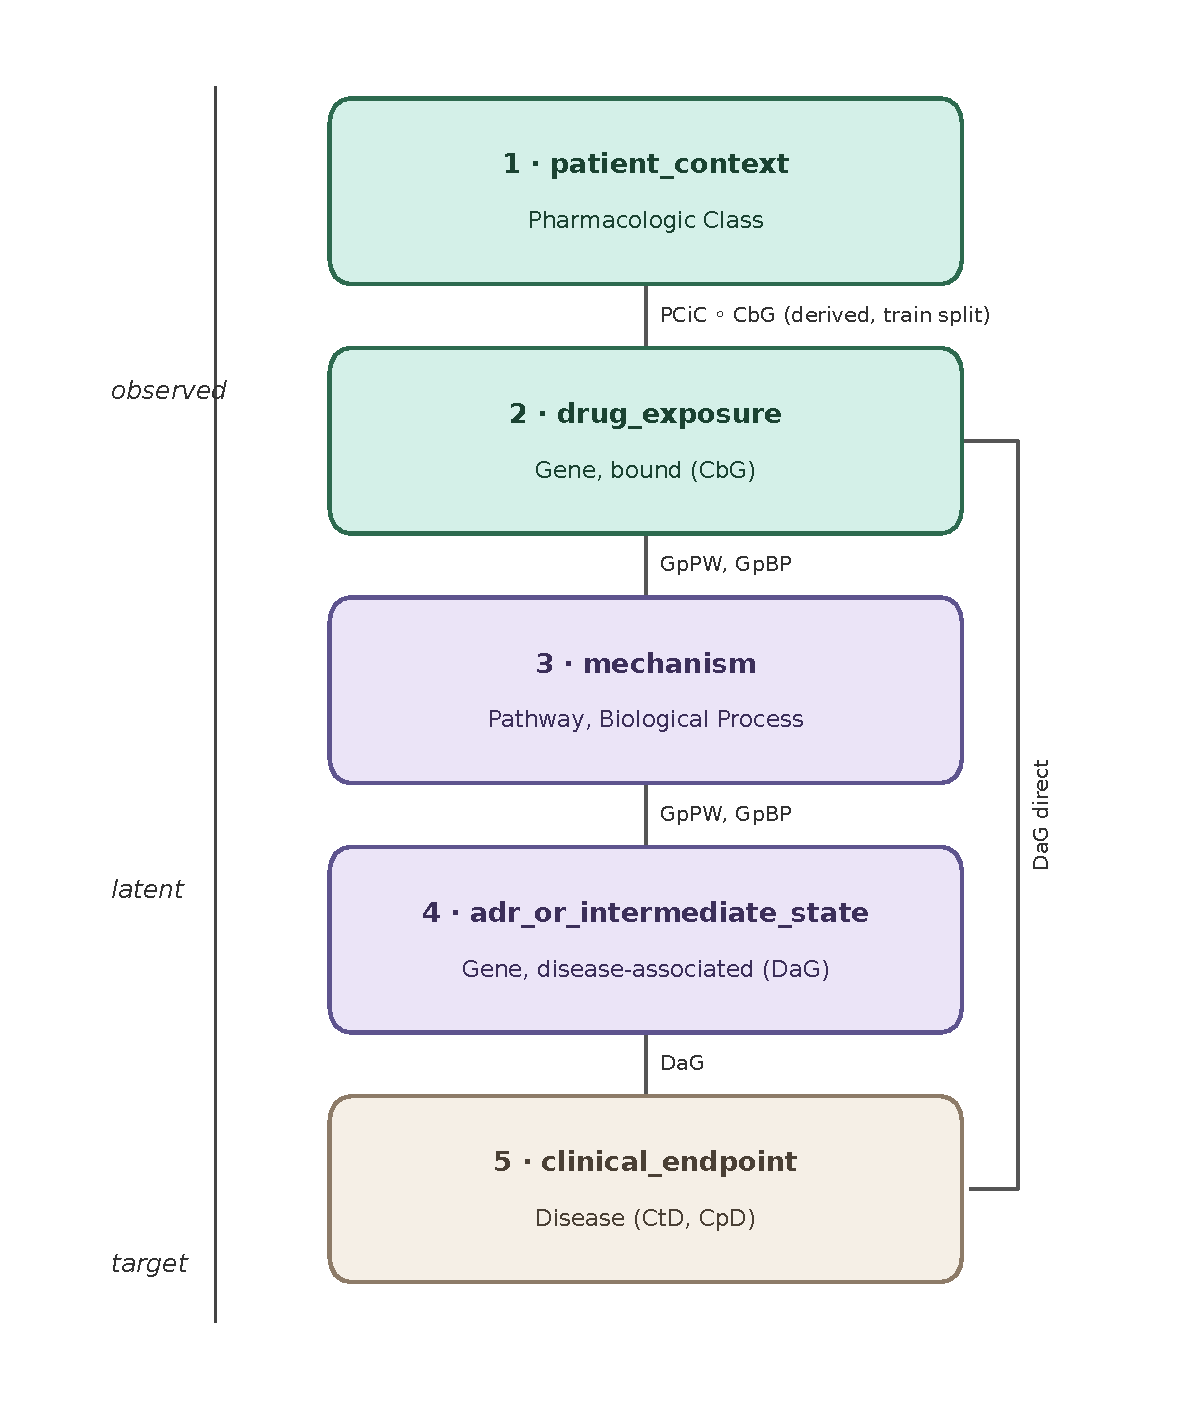
\includegraphics[width=0.92\textwidth,keepaspectratio]{rysunki/hetionet_layer_mapping.pdf}
  \caption{Hetionet layer mapping after reconstruction onto the synthetic schema.}
  \label{fig:updated_hetionet}
\end{figure}



\subsubsection{Results}

% The models on benchmark dataset shows the same trend as on synthethic dataset. 
% The approach with HCR significantly improves results comparing to baseline model without HCR. 
% It generates similar results as models with residual connections, but what it is interesting on the benchamrk dataset
% HCR combined with residual connections reaches the higher results than separated approach. 

The benchmark reproduces several trends
observed on the synthetic dataset---depth sensitivity without stabilisers,
partial recovery with HCR---under a different graph semantics and without
oracle metrics. The gain from HCR is conditional on the state of the
propagation path: at $L=6$ without
residual connections the baseline collapses to $0.585$ AUC on test, while every
HCR variant recovers a substantial part of it, up to $0.757$ for
\emph{typed+triple}. At $L=1$, where the receptive field of an endpoint
coincides with the input of the HCR branch, no variant improves on the
baseline, and the concatenated variants are slightly worse.

In the benchmark dataset, residual connections and HCR combine additively at
$L=6$. The baseline
reaches $0.585$ without either mechanism, $0.680$--$0.757$ with HCR alone,
$0.728$ with residual alone, and $0.760$ with both. The combination is
therefore better than either component in isolation.

The reason is the structure of the two graphs. In the synthetic graph the direct
parents of an endpoint are observed, so the statistical evidence branch and the one-hop
receptive field read the same variables and the two mechanisms address the same
bottleneck. In the Hetionet-derived graph depth is more crucial because some
layers are latent. Information must
therefore traverse several hops, and the residual path and the HCR bypass
contribute at different points of that route.

Overall, the proxy experiment suggests that combining message passing
with the statistical evidence branch remains useful with 
multi-hop reasoning. Whether an
additional residual path helps or hinders depends on where 
the statistical
evidence enters the model.


% =====================================================================
%  PROXY DATASET RESULTS (Hetionet, cut A, proxy3_clean)
%  1552 compounds, 20 endpoints, seed 42, conv_type = transformer,
%  hidden = 64, batch = 8, lr = 1e-3, dropedge = 0.0
% =====================================================================
\begin{table}[H]
  \centering
  \small
  \setlength{\tabcolsep}{4pt}
  \caption{Benchmark results for endpoint prediction.}
  \label{tab:proxy-full}
  \sisetup{table-format=1.3}
  \begin{tabular}{ccl SSS SSS}
    \toprule
    & & & \multicolumn{3}{c}{Validation} & \multicolumn{3}{c}{Test} \\
    \cmidrule(lr){4-6}\cmidrule(lr){7-9}
    $L$ & Res. & HCR & {AUC} & {AP} & {Lift} & {AUC} & {AP} & {Lift} \\
    \midrule
    1 & no  & ---              & 0.757 & 0.188 & 7.92  & 0.664 & 0.120 & 6.49 \\
    1 & no  & nonlin.\ bin.    & 0.763 & 0.207 & 8.75  & 0.657 & 0.120 & 6.47 \\
    1 & no  & nonlin.\ all     & 0.761 & 0.206 & 8.69  & 0.665 & 0.140 & 7.55 \\
    1 & no  & typed+triple     & 0.765 & 0.160 & 6.75  & 0.662 & 0.104 & 5.63 \\
    \addlinespace[2pt]
    1 & yes & ---              & 0.756 & 0.196 & 8.26  & 0.669 & 0.106 & 5.72 \\
    1 & yes & nonlin.\ bin.    & 0.756 & 0.201 & 8.49  & 0.670 & 0.135 & 7.31 \\
    1 & yes & nonlin.\ all     & 0.758 & 0.206 & 8.69  & 0.664 & 0.135 & 7.32 \\
    1 & yes & typed+triple     & 0.750 & 0.157 & 6.61  & 0.661 & 0.098 & 5.30 \\
    \midrule
    2 & no  & nonlin.\ all     & 0.763 & 0.263 & 11.10 & 0.694 & 0.173 & 9.34 \\
    2 & no  & typed+triple     & 0.778 & 0.263 & 11.10 & 0.677 & 0.175 & 9.46 \\
    \addlinespace[2pt]
    2 & yes & nonlin.\ all     & 0.760 & 0.224 & 9.44  & 0.684 & 0.154 & 8.31 \\
    2 & yes & typed+triple     & 0.765 & 0.232 & 9.79  & 0.690 & 0.174 & 9.43 \\
    \midrule
    3 & no  & ---              & 0.756 & 0.199 & 8.38  & 0.722 & 0.152 & 8.24 \\
    3 & no  & nonlin.\ bin.    & 0.805 & 0.275 & 11.62 & 0.686 & 0.169 & 9.14 \\
    3 & no  & nonlin.\ all     & 0.800 & 0.259 & 10.91 & 0.700 & 0.166 & 8.99 \\
    3 & no  & typed+triple     & 0.794 & 0.237 & 10.01 & 0.702 & 0.168 & 9.11 \\
    \addlinespace[2pt]
    3 & yes & ---              & 0.799 & 0.225 & 9.48  & 0.685 & 0.166 & 8.97 \\
    3 & yes & nonlin.\ bin.    & 0.814 & 0.235 & 9.90  & 0.714 & 0.183 & 9.92 \\
    3 & yes & nonlin.\ all     & 0.807 & 0.259 & 10.91 & 0.677 & 0.174 & 9.39 \\
    3 & yes & typed+triple     & 0.805 & 0.248 & 10.45 & 0.708 & 0.180 & 9.72 \\
    \midrule
    4 & no  & nonlin.\ all     & 0.757 & 0.230 & 9.70  & 0.678 & 0.151 & 8.14 \\
    4 & no  & typed+triple     & 0.807 & 0.262 & 11.06 & 0.747 & 0.181 & 9.79 \\
    \addlinespace[2pt]
    4 & yes & nonlin.\ all     & 0.814 & 0.238 & 10.05 & 0.715 & 0.180 & 9.76 \\
    4 & yes & typed+triple     & 0.806 & 0.240 & 10.12 & 0.713 & 0.168 & 9.06 \\
    \midrule
    5 & no  & nonlin.\ all     & 0.783 & 0.239 & 10.08 & 0.680 & 0.158 & 8.52 \\
    5 & no  & typed+triple     & 0.807 & 0.246 & 10.37 & 0.746 & 0.163 & 8.84 \\
    \addlinespace[2pt]
    5 & yes & nonlin.\ all     & 0.815 & 0.291 & 12.29 & 0.727 & 0.179 & 9.71 \\
    5 & yes & typed+triple     & 0.813 & 0.270 & 11.37 & 0.724 & 0.211 & 11.41 \\
    \midrule
    6 & no  & ---              & 0.610 & 0.121 & 5.11  & 0.585 & 0.077 & 4.14 \\
    6 & no  & nonlin.\ bin.    & 0.782 & 0.210 & 8.86  & 0.680 & 0.174 & 9.42 \\
    6 & no  & nonlin.\ all     & 0.794 & 0.237 & 9.99  & 0.682 & 0.157 & 8.51 \\
    6 & no  & typed+triple     & 0.803 & 0.263 & 11.11 & 0.757 & 0.175 & 9.45 \\
    \addlinespace[2pt]
    6 & yes & ---              & 0.817 & 0.255 & 10.77 & 0.728 & 0.173 & 9.36 \\
    6 & yes & nonlin.\ bin.    & 0.832 & 0.310 & 13.06 & 0.760 & 0.179 & 9.70 \\
    6 & yes & nonlin.\ all     & 0.812 & 0.235 & 9.92  & 0.734 & 0.166 & 8.96 \\
    6 & yes & typed+triple     & 0.808 & 0.251 & 10.59 & 0.730 & 0.205 & 11.10 \\
    \bottomrule
  \end{tabular}
\end{table}


% ---------------------------------------------------------------------
% TABLE 1 - full observability regime
% ---------------------------------------------------------------------
% \begin{table}[H]
%     \centering
%     \caption{Results under full observability on the proxy dataset. The
%       epoch was selected on the validation set. \texttt{---} in the HCR
%       column denotes a model without the HCR branch. Lift is AUPRC
%       divided by the prevalence baseline. Jumping knowledge was not used
%       in any configuration.}
%     \label{tab:proxy-full}
%     \sisetup{table-format=1.3}
%     \begin{tabular}{ccl SSS SSS}
%       \toprule
%       & & & \multicolumn{3}{c}{Validation} & \multicolumn{3}{c}{Test} \\
%       \cmidrule(lr){4-6}\cmidrule(lr){7-9}
%       $L$ & Residual & HCR & {AUC} & {AUPRC} & {Lift} & {AUC} & {AUPRC} & {Lift} \\
%       \midrule
%       1 & no  & ---            & 0.757 & 0.188 & 7.92  & 0.664 & 0.120 & 6.49 \\
%       1 & no  & nonlin.\ 9D    & 0.763 & 0.207 & 8.75  & 0.657 & 0.120 & 6.47 \\
%       1 & no  & typed 41D      & 0.759 & 0.194 & 8.17  & 0.663 & 0.116 & 6.29 \\
%       \addlinespace[2pt]
%       1 & yes & ---            & 0.756 & 0.196 & 8.26  & 0.669 & 0.106 & 5.72 \\
%       1 & yes & nonlin.\ 9D    & 0.756 & 0.201 & 8.49  & 0.670 & 0.135 & 7.31 \\
%       1 & yes & typed 41D      & 0.754 & 0.185 & 7.79  & 0.671 & 0.124 & 6.71 \\
%       \midrule
%       3 & no  & ---            & 0.756 & 0.199 & 8.38  & {\bfseries 0.722} & 0.152 & 8.24 \\
%       3 & no  & nonlin.\ 9D    & 0.805 & 0.275 & 11.62 & 0.686 & 0.169 & 9.14 \\
%       3 & no  & typed 41D      & 0.812 & 0.243 & 10.26 & 0.678 & 0.154 & 8.32 \\
%       \addlinespace[2pt]
%       3 & yes & ---            & 0.799 & 0.225 & 9.48  & 0.685 & 0.166 & 8.97 \\
%       3 & yes & nonlin.\ 9D    & 0.814 & 0.235 & 9.90  & 0.714 & 0.183 & 9.92 \\
%       3 & yes & typed 41D      & 0.802 & 0.255 & 10.76 & 0.678 & 0.151 & 8.16 \\
%       \midrule
%       6 & no  & ---            & 0.610 & 0.121 & 5.11  & 0.585 & 0.077 & 4.14 \\
%       6 & no  & nonlin.\ 9D    & 0.782 & 0.210 & 8.86  & 0.680 & 0.174 & 9.42 \\
%       6 & no  & typed 41D      & 0.794 & 0.235 & 9.89  & 0.680 & 0.126 & 6.84 \\
%       \addlinespace[2pt]
%       6 & yes & ---            & 0.817 & 0.255 & 10.77 & 0.728 & 0.173 & 9.36 \\
%       6 & yes & nonlin.\ 9D    & {\bfseries 0.832} & {\bfseries 0.310} & {\bfseries 13.06} & {\bfseries 0.760} & 0.179 & 9.70 \\
%       6 & yes & typed 41D      & 0.815 & 0.284 & 11.99 & 0.744 & {\bfseries 0.239} & {\bfseries 12.91} \\
%       \bottomrule
%     \end{tabular}
%   \end{table}
  
  
  % ---------------------------------------------------------------------
  % TABLE 3 - representation smoothing metrics
  % ---------------------------------------------------------------------
  % \begin{table}[H]
  %   \centering
  %   \caption{Representation smoothing metrics under full observability,
  %     measured on the validation set. By the conventional reading, lower
  %     MAD and higher cosine similarity indicate stronger smoothing.
  %     Validation AUC is repeated for comparison. Note that residual
  %     configurations appear more smoothed by every metric while
  %     performing better.}
  %   \label{tab:proxy-oversmoothing}
  %   \sisetup{table-format=1.4}
  %   \begin{tabular}{ccl SSSS S[table-format=1.3]}
  %     \toprule
  %     $L$ & Residual & HCR & {MAD} & {Cos.\ sim.} & {Cos.\ sim.\ (ep.)} & {Dirichlet} & {AUC} \\
  %     \midrule
  %     1 & no  & ---         & 0.7691 & 0.6216 & 0.8246 & 0.2706 & 0.757 \\
  %     1 & no  & nonlin.\ 9D & 0.7629 & 0.6142 & 0.7844 & 0.2495 & 0.763 \\
  %     1 & no  & typed 41D   & 0.7684 & 0.6191 & 0.8148 & 0.2706 & 0.759 \\
  %     \addlinespace[2pt]
  %     1 & yes & ---         & 0.7363 & 0.7042 & 0.7606 & 0.5724 & 0.756 \\
  %     1 & yes & nonlin.\ 9D & 0.7448 & 0.6946 & 0.7060 & 0.5048 & 0.756 \\
  %     1 & yes & typed 41D   & 0.7410 & 0.7026 & 0.7899 & 0.5022 & 0.754 \\
  %     \midrule
  %     3 & no  & ---         & 0.6515 & 0.6798 & 0.9582 & 0.1175 & 0.756 \\
  %     3 & no  & nonlin.\ 9D & 0.7067 & 0.6641 & 0.8365 & 0.0904 & 0.805 \\
  %     3 & no  & typed 41D   & 0.7235 & 0.6314 & 0.7333 & 0.0972 & 0.812 \\
  %     \addlinespace[2pt]
  %     3 & yes & ---         & 0.4842 & 0.8319 & 0.7772 & 0.3712 & 0.799 \\
  %     3 & yes & nonlin.\ 9D & 0.5517 & 0.7782 & 0.7752 & 0.3905 & 0.814 \\
  %     3 & yes & typed 41D   & 0.5113 & 0.8275 & 0.7132 & 0.4044 & 0.802 \\
  %     \midrule
  %     6 & no  & ---         & 0.7060 & 0.6530 & 0.8604 & 0.1024 & 0.610 \\
  %     6 & no  & nonlin.\ 9D & 0.7101 & 0.6495 & 0.7815 & 0.0892 & 0.782 \\
  %     6 & no  & typed 41D   & 0.7222 & 0.6408 & 0.8657 & 0.0949 & 0.794 \\
  %     \addlinespace[2pt]
  %     6 & yes & ---         & 0.5634 & 0.7975 & 0.7949 & 0.3143 & 0.817 \\
  %     6 & yes & nonlin.\ 9D & 0.5030 & 0.8174 & 0.6658 & 0.2636 & 0.832 \\
  %     6 & yes & typed 41D   & 0.5623 & 0.8095 & 0.8472 & 0.3930 & 0.815 \\
  %     \bottomrule
  %   \end{tabular}
  % \end{table}
\newpage % Rozdziały zaczynamy od nowej strony.
\section{Conclusions}

As a follow-up to the endpoint-prediction task, the following directions
could be pursued:

\begin{itemize}[label=\textendash]
  \item \textbf{Causal paths.}
  Greater emphasis could be placed on predictions along directed causal
  paths from drug exposure and patient context to clinical endpoints, together
  with a deeper analysis of what the model learns along those routes.

  \item \textbf{Real-world benchmarking.}
  Benchmarking the approach on MIMIC Clinical Database\footnote{%
    The MIMIC-III Clinical Database (v1.4) is a patient's dataset linking demographics, diagnoses, procedures, medications, and
    laboratory measurements that is used commonly in deep learning research.
    \url{https://physionet.org/content/mimiciii/1.4/}.%
  }
  could be a next step that would allow the pipeline to be validated on real clinical data.

  \item \textbf{GNN architectures.}
   Task~B was benchmarked with GraphSAGE, R-GCN, and TransformerConv; HGT was
    used in Task~A but not evaluated on endpoint prediction. A natural extension
    is to compare meta-relation attention (HGT) against TransformerConv on the
    same patient graph.

   \item \textbf{Statistical channel and HCR development.}
    Early experiments focused on pairwise dependence, while third-order evidence
    was implemented in a limited form, restricted to fully binary paths. Further
    work should devote more attention to triple-path evidence, and a dataset with
    richer numerical measurements at patient level would allow the Legendre
    expansion to be tested in larger scale.

  \item \textbf{Task~A--B loop.}
  Task~B currently uses a fixed graph; integrating it with Task~A link
  prediction would enable the closed-loop mechanism outlined in
  \cref{fig:loop}, in which graph updates and endpoint prediction inform one
  another iteratively.
\end{itemize}
%% Add to the main document where appendices should begin, usually after
% \bibliography{...} or \printbibliography:
%
% \appendix
% \input{appendix_data_generating_specification}
%
% If you use the `appendix` package and want a separate appendix page:
% \usepackage[toc,page]{appendix}  % preamble
% ...
% \begin{appendices}
% \input{appendix_data_generating_specification}
% \end{appendices}
%
% Required packages in the preamble:
% \usepackage{booktabs}
% \usepackage{tabularx}
% \usepackage{longtable}
% \usepackage{array}
%
% The tables below document variable classes and deterministic rules. The
% machine-readable files nodes.csv, edges.csv, and the generator source code
% remain the complete executable specification.

\texttt{Variable classes and generation mechanisms}


\begin{longtable}{@{}p{0.24\textwidth}p{0.12\textwidth}p{0.20\textwidth}p{0.34\textwidth}@{}}
\caption{Variable classes in the primary synthetic patient-level dataset.}
\label{tab:app_variable_classes} \\
\toprule
\textbf{Variable class} & \textbf{Number} & \textbf{Value type} & \textbf{Generation mechanism and role} \\
\midrule
\endfirsthead

\toprule
\textbf{Variable class} & \textbf{Number} & \textbf{Value type} & \textbf{Generation mechanism and role} \\
\midrule
\endhead

\bottomrule
\multicolumn{4}{r}{\emph{Continued on next page}} \\
\endfoot

\bottomrule
\endlastfoot

\texttt{patient\_id} & 1 & Integer & Unique technical patient identifier; not a graph node and not used as a predictive feature. \\
\addlinespace

\texttt{hospital\_id} & 1 & Categorical integer & Technical identifier of a simulated hospital. The primary \texttt{clean} scenario contains one hospital; multiple hospitals are used only in the \texttt{multihospital} extension. \\
\addlinespace

\texttt{patient\_context} & 24 & Mostly binary; selected count or baseline-measurement variables & Patient demographics, comorbidities, baseline clinical characteristics, latent severity, and treatment propensity. Values are initialised before downstream graph variables. \\
\addlinespace

\texttt{drug\_exposure} & 29 & Binary & Stochastic indicators of exposure to a drug class. Their probabilities are generated by the additive logistic model conditional on their direct graph parents. \\
\addlinespace

\texttt{mechanism} & 49 & Binary, count, and deterministic gate variables & Physiological mechanisms, interaction gates, drug-load variables, and other mediating concepts. Values are either sampled by the additive logistic model or calculated deterministically from their components. \\
\addlinespace

\texttt{adr\_or\_intermediate\_state} & 28 & Mostly binary; one derived score and one threshold variable & Intermediate adverse states and physiological consequences. Most are generated stochastically; \texttt{cumulative\_adr\_burden} and \texttt{severe\_adr\_burden} are deterministic derived variables. \\
\addlinespace

\texttt{observation\_or\_selection} & 12 & Binary & Variables representing testing, recording, reporting, or selection processes rather than the occurrence of a clinical state. \\
\addlinespace

\texttt{clinical\_endpoint} & 13 & Binary & Downstream clinical outcomes. Each is sampled from a Bernoulli distribution using a patient-specific probability conditional on its direct parents. These variables form the target labels for endpoint prediction. \\
\end{longtable}



\texttt{Deterministic variables}

\begin{longtable}{@{}p{0.30\textwidth}p{0.18\textwidth}p{0.42\textwidth}@{}}
\caption{Deterministic variables and their generating rules.}
\label{tab:app_deterministic_variables} \\
\toprule
\textbf{Variable} & \textbf{Rule type} & \textbf{Generating rule} \\
\midrule
\endfirsthead

\toprule
\textbf{Variable} & \textbf{Rule type} & \textbf{Generating rule} \\
\midrule
\endhead

\bottomrule
\multicolumn{3}{r}{\emph{Continued on next page}} \\
\endfoot

\bottomrule
\endlastfoot

\texttt{active\_drug\_count} & Drug count & Sum of all 29 binary \texttt{drug\_exposure} variables. \\
\addlinespace

\texttt{ddi\_renal\_double\_hit} & Conjunctive gate & \texttt{nsaid} $\land$ \texttt{acei\_arb}. \\
\addlinespace

\texttt{ddi\_renal\_triple\_whammy} & Conjunctive gate & \texttt{nsaid} $\land$ \texttt{acei\_arb} $\land$ \texttt{diuretic}. \\
\addlinespace

\texttt{ddi\_cns\_depression\_synergy} & Conjunctive gate & \texttt{opioid} $\land$ \texttt{benzodiazepine}. \\
\addlinespace

\texttt{ddi\_bleeding\_dual} & Conjunctive gate & \texttt{anticoagulant} $\land$ \texttt{antiplatelet}. \\
\addlinespace

\texttt{ddi\_bleeding\_triple} & Conjunctive gate & \texttt{nsaid} $\land$ \texttt{anticoagulant} $\land$ \texttt{antiplatelet}. \\
\addlinespace

\texttt{ddi\_serotonergic\_synergy} & Conjunctive gate & \texttt{ssri} $\land$ \texttt{snri}. \\
\addlinespace

\texttt{ddi\_hepatic\_triple\_hit} & Conjunctive gate & \texttt{hepatotoxic\_drug\_A} $\land$ \texttt{antibiotic\_hepatic\_risk} $\land$ \texttt{valproate\_like\_drug}. \\
\addlinespace

\texttt{ddi\_qt\_multidrug\_load} & Drug count & \texttt{qt\_prolonging\_drug} + \texttt{ssri} + \texttt{snri} + \texttt{macrolide} + \texttt{azole\_antifungal}. \\
\addlinespace

\texttt{nephrotoxin\_load} & Drug count & \texttt{nsaid} + \texttt{aminoglycoside} + \texttt{contrast\_agent} + \texttt{lithium} + \texttt{acei\_arb}. \\
\addlinespace

\texttt{hepatic\_drug\_load} & Drug count & \texttt{hepatotoxic\_drug\_A} + \texttt{antibiotic\_hepatic\_risk} + \texttt{valproate\_like\_drug} + \texttt{statin} + \texttt{macrolide} + \texttt{azole\_antifungal}. \\
\addlinespace

\texttt{qt\_drug\_load\_v3} & Drug count & \texttt{qt\_prolonging\_drug} + \texttt{ssri} + \texttt{snri} + \texttt{macrolide} + \texttt{azole\_antifungal} + \texttt{digoxin}. \\
\addlinespace

\texttt{cns\_depressant\_load} & Drug count & \texttt{opioid} + \texttt{benzodiazepine} + \texttt{anticholinergic} + \texttt{valproate\_like\_drug}. \\
\addlinespace

\texttt{bleeding\_risk\_load} & Drug count & \texttt{anticoagulant} + \texttt{antiplatelet} + \texttt{nsaid} + \texttt{ssri} + \texttt{corticosteroid}. \\
\addlinespace

\texttt{serotonergic\_load} & Drug count & \texttt{ssri} + \texttt{snri} + \texttt{opioid} + \texttt{triptan}. \\
\addlinespace

\texttt{cyp\_inhibitor\_load} & Drug count & \texttt{macrolide} + \texttt{azole\_antifungal}. \\
\addlinespace

\texttt{ddi\_statin\_cyp\_inhibitor} & Conjunctive gate & \texttt{statin} $\land$ $\mathbb{1}(\texttt{cyp\_inhibitor\_load} > 0)$. \\
\addlinespace

\texttt{ddi\_metformin\_renal\_risk} & Conjunctive gate & \texttt{metformin} $\land$ \texttt{ckd}. \\
\addlinespace

\texttt{ddi\_lithium\_renal\_risk} & Conjunctive gate & \texttt{lithium} $\land$ \texttt{ckd}. \\
\addlinespace

\texttt{ddi\_digoxin\_electrolyte\_risk} & Conjunctive gate & \texttt{digoxin} $\land$ \texttt{electrolyte\_disturbance}. \\
\addlinespace

\texttt{drug\_disease\_nsaid\_ckd} & Conjunctive gate & \texttt{nsaid} $\land$ \texttt{ckd}. \\
\addlinespace

\texttt{drug\_disease\_nsaid\_heart\_failure} & Conjunctive gate & \texttt{nsaid} $\land$ \texttt{heart\_failure}. \\
\addlinespace

\texttt{drug\_disease\_qt\_baseline\_risk} & Conjunctive gate & $\mathbb{1}(\texttt{qt\_drug\_load\_v3} > 0) \land$ \texttt{baseline\_qt\_risk}. \\
\addlinespace

\texttt{drug\_disease\_hepatic\_liver\_disease} & Conjunctive gate & $\mathbb{1}(\texttt{hepatic\_drug\_load} > 0) \land$ \texttt{liver\_disease}. \\
\addlinespace

\texttt{drug\_disease\_anticoagulant\_frailty} & Conjunctive gate & \texttt{anticoagulant} $\land$ \texttt{frailty}. \\
\addlinespace

\texttt{ddi\_serotonergic\_high\_load} & Threshold & $\mathbb{1}(\texttt{serotonergic\_load} \geq 2)$. \\
\addlinespace

\texttt{cumulative\_adr\_burden} & Weighted sum & $\sum_k \omega_k \cdot \texttt{ADR}_k + 0.08 \cdot \texttt{active\_drug\_count}$, where $\omega_k$ is the fixed severity weight for adverse-state component $k$. \\
\addlinespace

\texttt{severe\_adr\_burden} & Threshold & $\mathbb{1}(\texttt{cumulative\_adr\_burden} \geq 4.0)$. \\
\addlinespace

\texttt{elevated\_creatinine\_recorded} & Recorded-state rule & \texttt{creatinine\_rise} $\land$ \texttt{creatinine\_tested}. \\
\addlinespace

\texttt{elevated\_alt\_ast\_recorded} & Recorded-state rule & \texttt{alt\_ast\_rise} $\land$ \texttt{lft\_tested}. \\
\addlinespace

\texttt{qt\_recorded} & Recorded-state rule & \texttt{qt\_prolongation\_state} $\land$ \texttt{ecg\_performed}. \\
\end{longtable}





\cleardoublepage
\appendix{Appendix}
\label{appendix-list}
% Add to the main document where appendices should begin, usually after
% \bibliography{...} or \printbibliography:
%
% \appendix
% \input{appendix_data_generating_specification}
%
% If you use the `appendix` package and want a separate appendix page:
% \usepackage[toc,page]{appendix}  % preamble
% ...
% \begin{appendices}
% \input{appendix_data_generating_specification}
% \end{appendices}
%
% Required packages in the preamble:
% \usepackage{booktabs}
% \usepackage{tabularx}
% \usepackage{longtable}
% \usepackage{array}
%
% The tables below document variable classes and deterministic rules. The
% machine-readable files nodes.csv, edges.csv, and the generator source code
% remain the complete executable specification.

\texttt{Variable classes and generation mechanisms}


\begin{longtable}{@{}p{0.24\textwidth}p{0.12\textwidth}p{0.20\textwidth}p{0.34\textwidth}@{}}
\caption{Variable classes in the primary synthetic patient-level dataset.}
\label{tab:app_variable_classes} \\
\toprule
\textbf{Variable class} & \textbf{Number} & \textbf{Value type} & \textbf{Generation mechanism and role} \\
\midrule
\endfirsthead

\toprule
\textbf{Variable class} & \textbf{Number} & \textbf{Value type} & \textbf{Generation mechanism and role} \\
\midrule
\endhead

\bottomrule
\multicolumn{4}{r}{\emph{Continued on next page}} \\
\endfoot

\bottomrule
\endlastfoot

\texttt{patient\_id} & 1 & Integer & Unique technical patient identifier; not a graph node and not used as a predictive feature. \\
\addlinespace

\texttt{hospital\_id} & 1 & Categorical integer & Technical identifier of a simulated hospital. The primary \texttt{clean} scenario contains one hospital; multiple hospitals are used only in the \texttt{multihospital} extension. \\
\addlinespace

\texttt{patient\_context} & 24 & Mostly binary; selected count or baseline-measurement variables & Patient demographics, comorbidities, baseline clinical characteristics, latent severity, and treatment propensity. Values are initialised before downstream graph variables. \\
\addlinespace

\texttt{drug\_exposure} & 29 & Binary & Stochastic indicators of exposure to a drug class. Their probabilities are generated by the additive logistic model conditional on their direct graph parents. \\
\addlinespace

\texttt{mechanism} & 49 & Binary, count, and deterministic gate variables & Physiological mechanisms, interaction gates, drug-load variables, and other mediating concepts. Values are either sampled by the additive logistic model or calculated deterministically from their components. \\
\addlinespace

\texttt{adr\_or\_intermediate\_state} & 28 & Mostly binary; one derived score and one threshold variable & Intermediate adverse states and physiological consequences. Most are generated stochastically; \texttt{cumulative\_adr\_burden} and \texttt{severe\_adr\_burden} are deterministic derived variables. \\
\addlinespace

\texttt{observation\_or\_selection} & 12 & Binary & Variables representing testing, recording, reporting, or selection processes rather than the occurrence of a clinical state. \\
\addlinespace

\texttt{clinical\_endpoint} & 13 & Binary & Downstream clinical outcomes. Each is sampled from a Bernoulli distribution using a patient-specific probability conditional on its direct parents. These variables form the target labels for endpoint prediction. \\
\end{longtable}



\texttt{Deterministic variables}

\begin{longtable}{@{}p{0.30\textwidth}p{0.18\textwidth}p{0.42\textwidth}@{}}
\caption{Deterministic variables and their generating rules.}
\label{tab:app_deterministic_variables} \\
\toprule
\textbf{Variable} & \textbf{Rule type} & \textbf{Generating rule} \\
\midrule
\endfirsthead

\toprule
\textbf{Variable} & \textbf{Rule type} & \textbf{Generating rule} \\
\midrule
\endhead

\bottomrule
\multicolumn{3}{r}{\emph{Continued on next page}} \\
\endfoot

\bottomrule
\endlastfoot

\texttt{active\_drug\_count} & Drug count & Sum of all 29 binary \texttt{drug\_exposure} variables. \\
\addlinespace

\texttt{ddi\_renal\_double\_hit} & Conjunctive gate & \texttt{nsaid} $\land$ \texttt{acei\_arb}. \\
\addlinespace

\texttt{ddi\_renal\_triple\_whammy} & Conjunctive gate & \texttt{nsaid} $\land$ \texttt{acei\_arb} $\land$ \texttt{diuretic}. \\
\addlinespace

\texttt{ddi\_cns\_depression\_synergy} & Conjunctive gate & \texttt{opioid} $\land$ \texttt{benzodiazepine}. \\
\addlinespace

\texttt{ddi\_bleeding\_dual} & Conjunctive gate & \texttt{anticoagulant} $\land$ \texttt{antiplatelet}. \\
\addlinespace

\texttt{ddi\_bleeding\_triple} & Conjunctive gate & \texttt{nsaid} $\land$ \texttt{anticoagulant} $\land$ \texttt{antiplatelet}. \\
\addlinespace

\texttt{ddi\_serotonergic\_synergy} & Conjunctive gate & \texttt{ssri} $\land$ \texttt{snri}. \\
\addlinespace

\texttt{ddi\_hepatic\_triple\_hit} & Conjunctive gate & \texttt{hepatotoxic\_drug\_A} $\land$ \texttt{antibiotic\_hepatic\_risk} $\land$ \texttt{valproate\_like\_drug}. \\
\addlinespace

\texttt{ddi\_qt\_multidrug\_load} & Drug count & \texttt{qt\_prolonging\_drug} + \texttt{ssri} + \texttt{snri} + \texttt{macrolide} + \texttt{azole\_antifungal}. \\
\addlinespace

\texttt{nephrotoxin\_load} & Drug count & \texttt{nsaid} + \texttt{aminoglycoside} + \texttt{contrast\_agent} + \texttt{lithium} + \texttt{acei\_arb}. \\
\addlinespace

\texttt{hepatic\_drug\_load} & Drug count & \texttt{hepatotoxic\_drug\_A} + \texttt{antibiotic\_hepatic\_risk} + \texttt{valproate\_like\_drug} + \texttt{statin} + \texttt{macrolide} + \texttt{azole\_antifungal}. \\
\addlinespace

\texttt{qt\_drug\_load\_v3} & Drug count & \texttt{qt\_prolonging\_drug} + \texttt{ssri} + \texttt{snri} + \texttt{macrolide} + \texttt{azole\_antifungal} + \texttt{digoxin}. \\
\addlinespace

\texttt{cns\_depressant\_load} & Drug count & \texttt{opioid} + \texttt{benzodiazepine} + \texttt{anticholinergic} + \texttt{valproate\_like\_drug}. \\
\addlinespace

\texttt{bleeding\_risk\_load} & Drug count & \texttt{anticoagulant} + \texttt{antiplatelet} + \texttt{nsaid} + \texttt{ssri} + \texttt{corticosteroid}. \\
\addlinespace

\texttt{serotonergic\_load} & Drug count & \texttt{ssri} + \texttt{snri} + \texttt{opioid} + \texttt{triptan}. \\
\addlinespace

\texttt{cyp\_inhibitor\_load} & Drug count & \texttt{macrolide} + \texttt{azole\_antifungal}. \\
\addlinespace

\texttt{ddi\_statin\_cyp\_inhibitor} & Conjunctive gate & \texttt{statin} $\land$ $\mathbb{1}(\texttt{cyp\_inhibitor\_load} > 0)$. \\
\addlinespace

\texttt{ddi\_metformin\_renal\_risk} & Conjunctive gate & \texttt{metformin} $\land$ \texttt{ckd}. \\
\addlinespace

\texttt{ddi\_lithium\_renal\_risk} & Conjunctive gate & \texttt{lithium} $\land$ \texttt{ckd}. \\
\addlinespace

\texttt{ddi\_digoxin\_electrolyte\_risk} & Conjunctive gate & \texttt{digoxin} $\land$ \texttt{electrolyte\_disturbance}. \\
\addlinespace

\texttt{drug\_disease\_nsaid\_ckd} & Conjunctive gate & \texttt{nsaid} $\land$ \texttt{ckd}. \\
\addlinespace

\texttt{drug\_disease\_nsaid\_heart\_failure} & Conjunctive gate & \texttt{nsaid} $\land$ \texttt{heart\_failure}. \\
\addlinespace

\texttt{drug\_disease\_qt\_baseline\_risk} & Conjunctive gate & $\mathbb{1}(\texttt{qt\_drug\_load\_v3} > 0) \land$ \texttt{baseline\_qt\_risk}. \\
\addlinespace

\texttt{drug\_disease\_hepatic\_liver\_disease} & Conjunctive gate & $\mathbb{1}(\texttt{hepatic\_drug\_load} > 0) \land$ \texttt{liver\_disease}. \\
\addlinespace

\texttt{drug\_disease\_anticoagulant\_frailty} & Conjunctive gate & \texttt{anticoagulant} $\land$ \texttt{frailty}. \\
\addlinespace

\texttt{ddi\_serotonergic\_high\_load} & Threshold & $\mathbb{1}(\texttt{serotonergic\_load} \geq 2)$. \\
\addlinespace

\texttt{cumulative\_adr\_burden} & Weighted sum & $\sum_k \omega_k \cdot \texttt{ADR}_k + 0.08 \cdot \texttt{active\_drug\_count}$, where $\omega_k$ is the fixed severity weight for adverse-state component $k$. \\
\addlinespace

\texttt{severe\_adr\_burden} & Threshold & $\mathbb{1}(\texttt{cumulative\_adr\_burden} \geq 4.0)$. \\
\addlinespace

\texttt{elevated\_creatinine\_recorded} & Recorded-state rule & \texttt{creatinine\_rise} $\land$ \texttt{creatinine\_tested}. \\
\addlinespace

\texttt{elevated\_alt\_ast\_recorded} & Recorded-state rule & \texttt{alt\_ast\_rise} $\land$ \texttt{lft\_tested}. \\
\addlinespace

\texttt{qt\_recorded} & Recorded-state rule & \texttt{qt\_prolongation\_state} $\land$ \texttt{ecg\_performed}. \\
\end{longtable}





\cleardoublepage % Zaczynamy od nieparzystej strony
\printbibliography


% Spisy (opcjonalne)
\newpage
\pagestyle{plain}

\vspace{0.8cm}


\listoffigurestoc
\vspace{1cm}
\listoftablestoc

\end{document}